\PassOptionsToPackage{unicode=true}{hyperref} % options for packages loaded elsewhere
\PassOptionsToPackage{hyphens}{url}
%
\documentclass[]{book}
\usepackage{lmodern}
\usepackage{amssymb,amsmath}
\usepackage{ifxetex,ifluatex}
\usepackage{fixltx2e} % provides \textsubscript
\ifnum 0\ifxetex 1\fi\ifluatex 1\fi=0 % if pdftex
  \usepackage[T1]{fontenc}
  \usepackage[utf8]{inputenc}
  \usepackage{textcomp} % provides euro and other symbols
\else % if luatex or xelatex
  \usepackage{unicode-math}
  \defaultfontfeatures{Ligatures=TeX,Scale=MatchLowercase}
\fi
% use upquote if available, for straight quotes in verbatim environments
\IfFileExists{upquote.sty}{\usepackage{upquote}}{}
% use microtype if available
\IfFileExists{microtype.sty}{%
\usepackage[]{microtype}
\UseMicrotypeSet[protrusion]{basicmath} % disable protrusion for tt fonts
}{}
\IfFileExists{parskip.sty}{%
\usepackage{parskip}
}{% else
\setlength{\parindent}{0pt}
\setlength{\parskip}{6pt plus 2pt minus 1pt}
}
\usepackage{hyperref}
\hypersetup{
            pdftitle={Outstanding User Interfaces with Shiny},
            pdfauthor={David Granjon},
            pdfborder={0 0 0},
            breaklinks=true}
\urlstyle{same}  % don't use monospace font for urls
\usepackage{color}
\usepackage{fancyvrb}
\newcommand{\VerbBar}{|}
\newcommand{\VERB}{\Verb[commandchars=\\\{\}]}
\DefineVerbatimEnvironment{Highlighting}{Verbatim}{commandchars=\\\{\}}
% Add ',fontsize=\small' for more characters per line
\usepackage{framed}
\definecolor{shadecolor}{RGB}{248,248,248}
\newenvironment{Shaded}{\begin{snugshade}}{\end{snugshade}}
\newcommand{\AlertTok}[1]{\textcolor[rgb]{0.94,0.16,0.16}{#1}}
\newcommand{\AnnotationTok}[1]{\textcolor[rgb]{0.56,0.35,0.01}{\textbf{\textit{#1}}}}
\newcommand{\AttributeTok}[1]{\textcolor[rgb]{0.77,0.63,0.00}{#1}}
\newcommand{\BaseNTok}[1]{\textcolor[rgb]{0.00,0.00,0.81}{#1}}
\newcommand{\BuiltInTok}[1]{#1}
\newcommand{\CharTok}[1]{\textcolor[rgb]{0.31,0.60,0.02}{#1}}
\newcommand{\CommentTok}[1]{\textcolor[rgb]{0.56,0.35,0.01}{\textit{#1}}}
\newcommand{\CommentVarTok}[1]{\textcolor[rgb]{0.56,0.35,0.01}{\textbf{\textit{#1}}}}
\newcommand{\ConstantTok}[1]{\textcolor[rgb]{0.00,0.00,0.00}{#1}}
\newcommand{\ControlFlowTok}[1]{\textcolor[rgb]{0.13,0.29,0.53}{\textbf{#1}}}
\newcommand{\DataTypeTok}[1]{\textcolor[rgb]{0.13,0.29,0.53}{#1}}
\newcommand{\DecValTok}[1]{\textcolor[rgb]{0.00,0.00,0.81}{#1}}
\newcommand{\DocumentationTok}[1]{\textcolor[rgb]{0.56,0.35,0.01}{\textbf{\textit{#1}}}}
\newcommand{\ErrorTok}[1]{\textcolor[rgb]{0.64,0.00,0.00}{\textbf{#1}}}
\newcommand{\ExtensionTok}[1]{#1}
\newcommand{\FloatTok}[1]{\textcolor[rgb]{0.00,0.00,0.81}{#1}}
\newcommand{\FunctionTok}[1]{\textcolor[rgb]{0.00,0.00,0.00}{#1}}
\newcommand{\ImportTok}[1]{#1}
\newcommand{\InformationTok}[1]{\textcolor[rgb]{0.56,0.35,0.01}{\textbf{\textit{#1}}}}
\newcommand{\KeywordTok}[1]{\textcolor[rgb]{0.13,0.29,0.53}{\textbf{#1}}}
\newcommand{\NormalTok}[1]{#1}
\newcommand{\OperatorTok}[1]{\textcolor[rgb]{0.81,0.36,0.00}{\textbf{#1}}}
\newcommand{\OtherTok}[1]{\textcolor[rgb]{0.56,0.35,0.01}{#1}}
\newcommand{\PreprocessorTok}[1]{\textcolor[rgb]{0.56,0.35,0.01}{\textit{#1}}}
\newcommand{\RegionMarkerTok}[1]{#1}
\newcommand{\SpecialCharTok}[1]{\textcolor[rgb]{0.00,0.00,0.00}{#1}}
\newcommand{\SpecialStringTok}[1]{\textcolor[rgb]{0.31,0.60,0.02}{#1}}
\newcommand{\StringTok}[1]{\textcolor[rgb]{0.31,0.60,0.02}{#1}}
\newcommand{\VariableTok}[1]{\textcolor[rgb]{0.00,0.00,0.00}{#1}}
\newcommand{\VerbatimStringTok}[1]{\textcolor[rgb]{0.31,0.60,0.02}{#1}}
\newcommand{\WarningTok}[1]{\textcolor[rgb]{0.56,0.35,0.01}{\textbf{\textit{#1}}}}
\usepackage{longtable,booktabs}
% Fix footnotes in tables (requires footnote package)
\IfFileExists{footnote.sty}{\usepackage{footnote}\makesavenoteenv{longtable}}{}
\usepackage{graphicx,grffile}
\makeatletter
\def\maxwidth{\ifdim\Gin@nat@width>\linewidth\linewidth\else\Gin@nat@width\fi}
\def\maxheight{\ifdim\Gin@nat@height>\textheight\textheight\else\Gin@nat@height\fi}
\makeatother
% Scale images if necessary, so that they will not overflow the page
% margins by default, and it is still possible to overwrite the defaults
% using explicit options in \includegraphics[width, height, ...]{}
\setkeys{Gin}{width=\maxwidth,height=\maxheight,keepaspectratio}
\setlength{\emergencystretch}{3em}  % prevent overfull lines
\providecommand{\tightlist}{%
  \setlength{\itemsep}{0pt}\setlength{\parskip}{0pt}}
\setcounter{secnumdepth}{5}
% Redefines (sub)paragraphs to behave more like sections
\ifx\paragraph\undefined\else
\let\oldparagraph\paragraph
\renewcommand{\paragraph}[1]{\oldparagraph{#1}\mbox{}}
\fi
\ifx\subparagraph\undefined\else
\let\oldsubparagraph\subparagraph
\renewcommand{\subparagraph}[1]{\oldsubparagraph{#1}\mbox{}}
\fi

% set default figure placement to htbp
\makeatletter
\def\fps@figure{htbp}
\makeatother

\usepackage{booktabs}
\usepackage{amsthm}
\makeatletter
\def\thm@space@setup{%
  \thm@preskip=8pt plus 2pt minus 4pt
  \thm@postskip=\thm@preskip
}
\makeatother
\usepackage[]{natbib}
\bibliographystyle{apalike}

\title{Outstanding User Interfaces with Shiny}
\author{David Granjon}
\date{2020-05-11}

\begin{document}
\maketitle

{
\setcounter{tocdepth}{1}
\tableofcontents
}
\hypertarget{prerequisites}{%
\chapter*{Prerequisites}\label{prerequisites}}
\addcontentsline{toc}{chapter}{Prerequisites}

\begin{itemize}
\tightlist
\item
  Be familiar with \href{https://mastering-shiny.org}{Shiny}
\item
  Basic knowledge in HTML and JavaScript is a plus but not mandatory
\end{itemize}

\hypertarget{disclaimer}{%
\section*{Disclaimer}\label{disclaimer}}
\addcontentsline{toc}{section}{Disclaimer}

This book is not an HTML/Javascript/CSS course! Instead, it provides a \emph{survival kit} to be able to customize Shiny. I am sure however that readers will want to explore more about these topics.

\hypertarget{is-this-book-for-me}{%
\section*{Is this book for me?}\label{is-this-book-for-me}}
\addcontentsline{toc}{section}{Is this book for me?}

You should read this book if you answer yes to the following questions:

\begin{itemize}
\tightlist
\item
  Do you want to know how to develop outstanding shiny apps?
\item
  Have you ever wondered how to develop new input widgets?
\end{itemize}

\hypertarget{related-content}{%
\section*{Related content}\label{related-content}}
\addcontentsline{toc}{section}{Related content}

See the \href{https://rstudio.cloud}{RStudio Cloud} dedicated project.

\begin{Shaded}
\begin{Highlighting}[]
\KeywordTok{library}\NormalTok{(shiny)}
\KeywordTok{library}\NormalTok{(shinydashboard)}
\KeywordTok{library}\NormalTok{(shiny.semantic)}
\KeywordTok{library}\NormalTok{(cascadess)}
\KeywordTok{library}\NormalTok{(htmltools)}
\KeywordTok{library}\NormalTok{(purrr)}
\KeywordTok{library}\NormalTok{(magrittr)}
\end{Highlighting}
\end{Shaded}

\hypertarget{intro}{%
\chapter{Introduction}\label{intro}}

There are various Shiny focused resources introducing basic as well as advanced topics such as modules and Javascript/R interactions. However, handling advanced user interfaces was never an emphasis. Clients often desire custom designs, yet this generally exceeds core features of Shiny. We recognized that R App developers lacking a significant background in web development may have found this requirement to be overwhelming. Consequently, the aim of this book is to provide readers the necessary knowledge to extend Shiny's layout, input widgets and output elements. This book is organized into four parts. We first go through the basics of HTML, JavaScript and jQuery. In part 2, we dive into the \{htmltools\} package, providing functions to create and manipulate shiny tags as well as manage dependencies. Part 3 homes in on the development of a new template on top of Shiny by demonstrating examples from the \{bs4Dash\} and \{shinyMobile\} packages, part of the RinteRface project.

\hypertarget{part-survival-kit}{%
\part*{Survival Kit}\label{part-survival-kit}}
\addcontentsline{toc}{part}{Survival Kit}

This part will give you basis in HTML, JavaScript to get started\ldots{}

\hypertarget{survival-kit-html}{%
\chapter{HTML}\label{survival-kit-html}}

In the following, we will give a short introduction to the HTML language. First of all, let's do the following experience:

\begin{itemize}
\tightlist
\item
  Open your RStudio IDE
\item
  Load shiny with \texttt{library(shiny)}
\item
  Execute \texttt{p("Hello\ World")} and notice the output format
\item
  This is an HTML tag!
\end{itemize}

\hypertarget{html-basics}{%
\section{HTML Basics}\label{html-basics}}

HTML (Hypertext Markup Language) is derived from the SGML (Standard Generalized markup Language). An HTML file contains tags that can be divided into 2 catagories:

\begin{itemize}
\tightlist
\item
  paired-tags
\item
  closing-tags
\end{itemize}

\begin{Shaded}
\begin{Highlighting}[]
\CommentTok{<!-- /* paired-tags */ -->}
\KeywordTok{<p></p>}
\KeywordTok{<div></div>}

\CommentTok{<!-- /* self-closing tags */ -->}
\KeywordTok{<iframe/>}
\KeywordTok{<img/>}
\KeywordTok{<input/>}
\KeywordTok{<br/>}
\end{Highlighting}
\end{Shaded}

\hypertarget{tag-attributes}{%
\section{Tag attributes}\label{tag-attributes}}

All tags above don't have any attributes. Yet HTML allows to set attributes inside each tag. There exist a large range of attributes and we will only see 2 of them for now:

\begin{itemize}
\tightlist
\item
  class: may be shared between multiple tags
\item
  id: each must be unique
\end{itemize}

\begin{Shaded}
\begin{Highlighting}[]
\KeywordTok{<div}\OtherTok{ class=}\StringTok{"awesome-item"}\OtherTok{ id=}\StringTok{"myitem"}\KeywordTok{></div>}
\CommentTok{<!-- /* the class awesome-item may be applied to multiple tags */ -->}
\KeywordTok{<span}\OtherTok{ class=}\StringTok{"awesome-item"}\KeywordTok{></span>}
\end{Highlighting}
\end{Shaded}

Both attributes are widely used by CSS and JavaScript (we will discover in the following chapter the jQuery selectors) to apply custom style to a web page. While class may apply to multiple elements, id is restricted to only one item.

\hypertarget{html-page-skeleton}{%
\section{HTML page: skeleton}\label{html-page-skeleton}}

An HTML page is a collection of tags which will be interpreted by the web browser step by step. The simplest HTML page may be defined as follows:

\begin{Shaded}
\begin{Highlighting}[]
\DataTypeTok{<!DOCTYPE }\NormalTok{HTML}\DataTypeTok{>}
\KeywordTok{<html>}
  \KeywordTok{<head>}
  \CommentTok{<!-- /* head content here */ -->}
  \KeywordTok{</head>}
  \KeywordTok{<body>}
  \CommentTok{<!-- /* body content here */ -->}
  \KeywordTok{</body>}
\KeywordTok{</html>}
\end{Highlighting}
\end{Shaded}

\begin{itemize}
\tightlist
\item
  \texttt{\textless{}html\textgreater{}} is the may wrapper
\item
  \texttt{\textless{}head\textgreater{}} and \texttt{\textless{}body\textgreater{}} are the 2 main children
\end{itemize}

\texttt{\textless{}head\textgreater{}} contains dependencies like styles and JavaScript files (but not only), \texttt{\textless{}body\textgreater{}} contains the page content. We will see later that JavaScript files are often added just before the end of the \texttt{\textless{}body\textgreater{}}.

Only the body content is displayed on the screen!

Let's write the famous Hello World in html:

\begin{Shaded}
\begin{Highlighting}[]
\DataTypeTok{<!DOCTYPE }\NormalTok{HTML}\DataTypeTok{>}
\KeywordTok{<html>}
  \KeywordTok{<head>}
  \CommentTok{<!-- head content here -->}
  \KeywordTok{</head>}
  \KeywordTok{<body>}
  \KeywordTok{<p>}\NormalTok{Hello World}\KeywordTok{</p>}
  \KeywordTok{</body>}
\KeywordTok{</html>}
\end{Highlighting}
\end{Shaded}

In order to preview this page in a web browser, you need to save the above snippet to a script \texttt{hello-world.html} and double-click on it. It will open with you default web browser.

\hypertarget{about-the-dom}{%
\section{About the DOM}\label{about-the-dom}}

The DOM stands for ``Document Object Model'', is a convenient representation of the html document. There actually exists multiple DOM types, namely DOM-XML and DOM-HTML but we will only focus on the later (in the following DOM is DOM-HTML).
If we consider the last example (Hello World), the associated DOM tree may be inspected in Figure \ref{fig:html-dom}.

\hypertarget{visualizing-the-dom-the-html-inspector}{%
\subsection{Visualizing the DOM: the HTML inspector}\label{visualizing-the-dom-the-html-inspector}}

Below, we introduce a tool that we is going to be a valuable ally during our ambitious quest to beautiful shiny user interfaces. In this chapter, we restrict the description to the first panel of the HTML inspector \footnote{As shown in Figure \ref{fig:html-dom}, the inspector also has tools to debug JavaScript code, inspect files, run performances audit, \ldots{} We will describe some of these later in the book.}. This feature is available in all web browser but we will only focus on Chrome.

\begin{itemize}
\tightlist
\item
  Open the hello-world.html example in a web browser (google chrome here)
\item
  Right-click to open the HTML inspector (developer tools must be enabled if it is not the case)
\end{itemize}

The HTML inspector in a convenient tool to explore the structure of the current HTML page. On the left-hand side, the DOM tree is displayed and we clearly see that \texttt{\textless{}html\textgreater{}} is the parent of \texttt{\textless{}head\textgreater{}} and \texttt{\textless{}body\textgreater{}}. \texttt{\textless{}body\textgreater{}} has also 1 child, that is \texttt{\textless{}p\textgreater{}}. We didn't mention this yet but we can preview any style (CSS) associated to the selected element on the right panel as well as Event Listeners (JavaScript). We will discuss that in the next chapter.

\begin{figure}
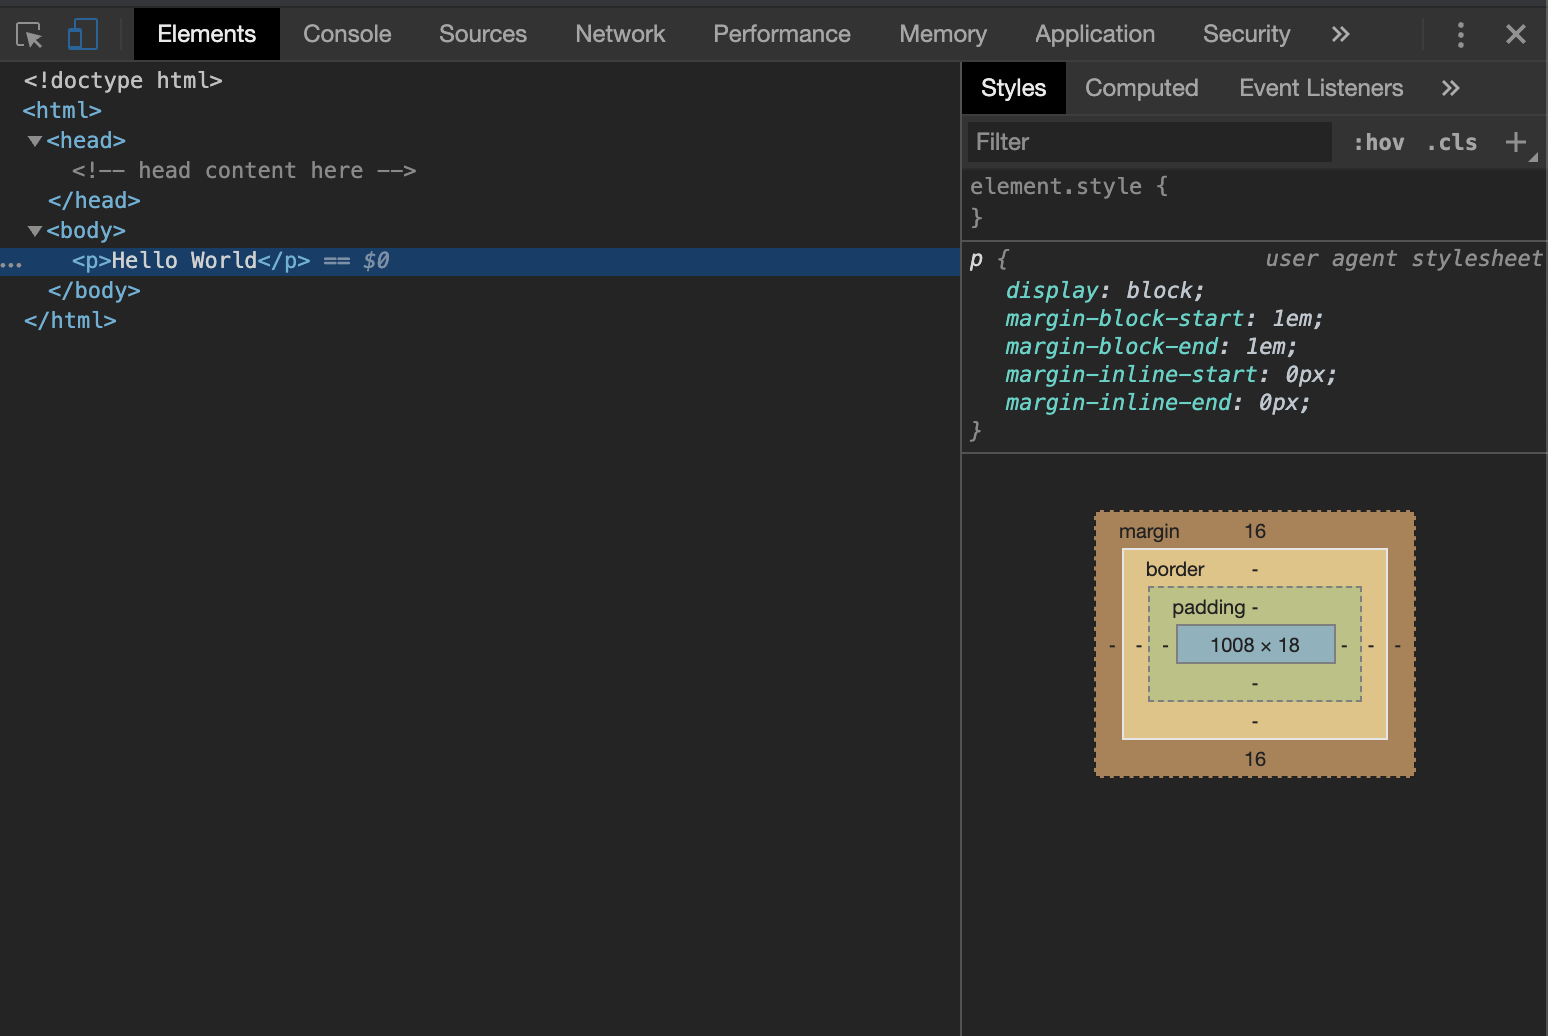
\includegraphics[width=21.5in]{images/survival-kit/dom} \caption{Inspection of the DOM in the Hello World example}\label{fig:html-dom}
\end{figure}

\hypertarget{preliminary-introduction-to-css-and-javascript}{%
\section{Preliminary introduction to CSS and JavaScript}\label{preliminary-introduction-to-css-and-javascript}}

CSS and JavaScript are tools to enhance an HTML page.

\hypertarget{html-and-css}{%
\subsection{HTML and CSS}\label{html-and-css}}

CSS (Cascading Style Sheets) changes the style of HTML tags by targeting specific classes or ids. For instance, if we want all p tags to have red color we will use:

\begin{Shaded}
\begin{Highlighting}[]
\NormalTok{p \{}
  \KeywordTok{color}\NormalTok{: }\DecValTok{red}\NormalTok{;}
\NormalTok{\}}
\end{Highlighting}
\end{Shaded}

To include CSS in an HTML page, we use the \texttt{\textless{}style\textgreater{}} tag as follows:

\begin{Shaded}
\begin{Highlighting}[]
\DataTypeTok{<!DOCTYPE }\NormalTok{HTML}\DataTypeTok{>}
\KeywordTok{<html>}
  \KeywordTok{<head>}
    \KeywordTok{<style}\OtherTok{ type=}\StringTok{"text/css"}\KeywordTok{>}
\NormalTok{      p \{}
        \KeywordTok{color}\NormalTok{: }\DecValTok{red}\NormalTok{;}
\NormalTok{      \}}
    \KeywordTok{</style>}
  \KeywordTok{</head>}
  \KeywordTok{<body>}
  \KeywordTok{<p>}\NormalTok{Hello World}\KeywordTok{</p>}
  \KeywordTok{</body>}
\KeywordTok{</html>}
\end{Highlighting}
\end{Shaded}

You may update the hello-world.html script and run it in your web-browser to see the difference (this is not super impressive but a good start). There exist other ways to include CSS (see next chapters).

\hypertarget{html-and-javascript}{%
\subsection{HTML and JavaScript}\label{html-and-javascript}}

JavaScript is also going to be one of our best friend in this book.
You will see how quickly/seamlessly you may add awesome feature to your shiny app.

Let's consider an example below:

\begin{Shaded}
\begin{Highlighting}[]
\DataTypeTok{<!DOCTYPE }\NormalTok{HTML}\DataTypeTok{>}
\KeywordTok{<html>}
  \KeywordTok{<head>}
    \KeywordTok{<style}\OtherTok{ type=}\StringTok{"text/css"}\KeywordTok{>}
\NormalTok{      p \{}
        \KeywordTok{color}\NormalTok{: }\DecValTok{red}\NormalTok{;}
\NormalTok{      \}}
    \KeywordTok{</style>}
    \KeywordTok{<script}\OtherTok{ language=}\StringTok{"javascript"}\KeywordTok{>}
      \CommentTok{// displays an alert }
      \AttributeTok{alert}\NormalTok{(}\StringTok{'Click on the Hello World text!'}\NormalTok{)}\OperatorTok{;}
      \CommentTok{// change text color}
      \KeywordTok{function} \AttributeTok{changeColor}\NormalTok{(color)}\OperatorTok{\{}
        \VariableTok{document}\NormalTok{.}\AttributeTok{getElementById}\NormalTok{(}\StringTok{'hello'}\NormalTok{).}\VariableTok{style}\NormalTok{.}\AttributeTok{color} \OperatorTok{=} \StringTok{"green"}\OperatorTok{;}
      \OperatorTok{\}}
    \KeywordTok{</script>}
  \KeywordTok{</head>}
  \KeywordTok{<body>}
    \CommentTok{<!-- onclick attributes applies the JavaScript function changeColor define above -->}
    \KeywordTok{<p}\OtherTok{ id=}\StringTok{"hello"}\OtherTok{ onclick=}\StringTok{"changeColor('green')"}\KeywordTok{>}\NormalTok{Hello World}\KeywordTok{</p>}
  \KeywordTok{</body>}
\KeywordTok{</html>}
\end{Highlighting}
\end{Shaded}

In few lines of code, you can change the color of the text. Wonderful isn'it?
Let's move to the next chapter to discover JavaScript!

\hypertarget{survival-kit-javascript}{%
\chapter{JavaScript}\label{survival-kit-javascript}}

\hypertarget{introduction}{%
\section{Introduction}\label{introduction}}

JavaScript (JS) was created in 1995 by Brendan Eich and also known as ECMAScript (ES). Interestingly, you might have heard about ActionScript, which is no more than an implementation of ES by Adobe Systems. Nowadays, JavaScript is a centerpiece of the web and included in almost all websites.

Let's make a little experiment. If you have a personal blog (it is very popular in the RStats community) you probably know Hugo or Jekyll. These tools allow to quickly setup professionnal looking (or at least not too ugly) blogs in literraly few minutes. You can focus on the content and this is what matters! Now, if you open the HTML inspector introduced in Chapter \ref{survival-kit-html}, click on the elements tab (in theory it is the first tab and open by default), and uncollapse the \texttt{\textless{}head\textgreater{}} tag, you see that a lot of scripts are included, as shown in Figure \ref{fig:scripts-list}. Same remark in the \texttt{\textless{}body\textgreater{}} tag.

\begin{figure}
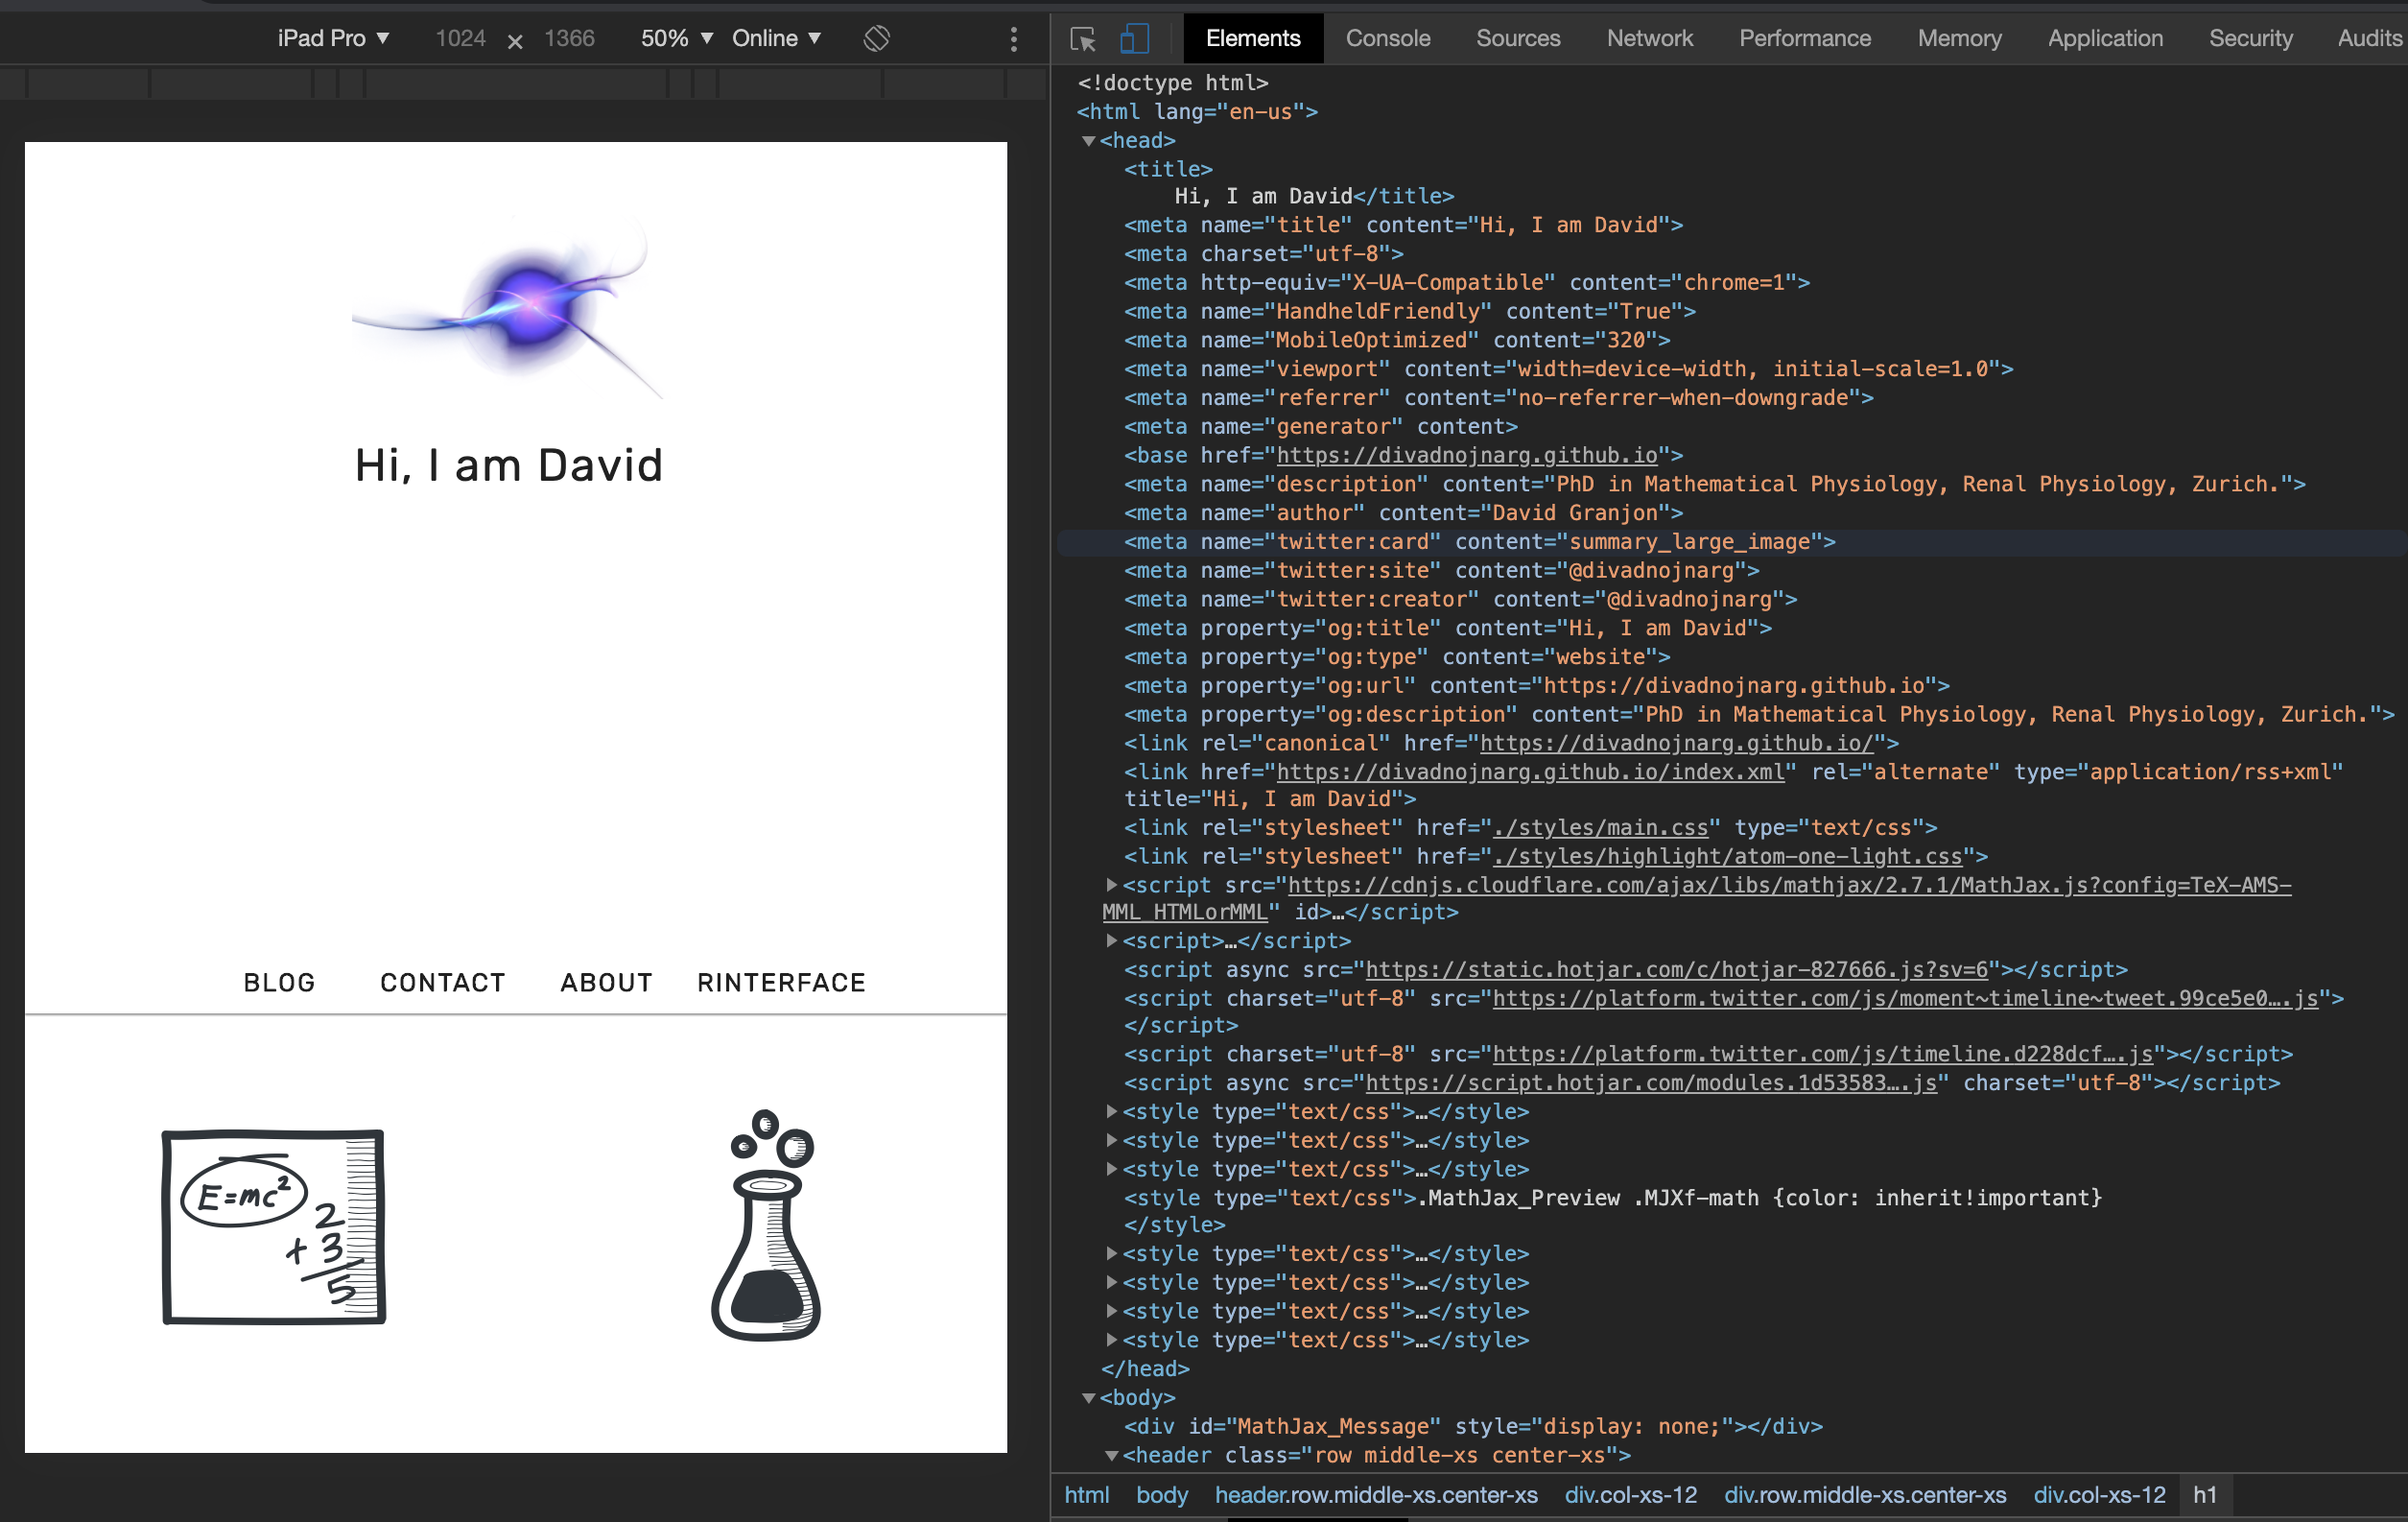
\includegraphics[width=34.86in]{images/survival-kit/scripts-list} \caption{A website is full of JavaScript}\label{fig:scripts-list}
\end{figure}

There are 2 main ways to include scripts:

\begin{itemize}
\tightlist
\item
  Use the \texttt{\textless{}script\textgreater{}} tag with the JS code inside
\item
  Import an external file containing the JS code and only
\end{itemize}

\begin{Shaded}
\begin{Highlighting}[]
\KeywordTok{<script}\OtherTok{ type=}\StringTok{"text/javascript"}\KeywordTok{>}
\CommentTok{// JS code here}
\KeywordTok{</script>}
\end{Highlighting}
\end{Shaded}

\begin{Shaded}
\begin{Highlighting}[]
\CommentTok{<!-- We use the src attribute to link the external file -->}
\KeywordTok{<script}\OtherTok{ type=}\StringTok{"text/javascript"}\OtherTok{ src=}\StringTok{"file.js"}\KeywordTok{>}
\end{Highlighting}
\end{Shaded}

Whether to choose the first or second method depends on the content of your script. If we consider jQuery, a well known JS library, it contains so much lines of code that it does not make sense to select the first method.

\hypertarget{setup}{%
\section{Setup}\label{setup}}

Like R or Python, JavaScript is an interpreted language. It is also executed client side, that is in the navigator. It also means that you cannot run js code without suitable tools.

\hypertarget{node}{%
\subsection{Node}\label{node}}

\href{https://nodejs.org/en/}{Node} contains an interpreter for JS as well as a dependencies manager, npm (Node Package Manager). To install Node on your computer, browse to the website and follow the intruction. Once done, open a terminal and check if

\begin{verbatim}
$ which node
$ node --version
\end{verbatim}

returns something. If not, it means that Node is not properly installed.

\hypertarget{choose-a-good-ide}{%
\subsection{Choose a good IDE}\label{choose-a-good-ide}}

I really like \href{https://code.visualstudio.com}{VSCode} for all the JS things since it contains a Node interpreter and you can seamlessly execute any JS code (the truth is because I'm a big fan of the dracula color theme). But the \href{https://rstudio.com/products/rstudio/}{Rstudio IDE} may also be fine, provided that you have Node installed. Below, we will see how to run a JS code in both IDE.

\hypertarget{first-script}{%
\subsection{First Script}\label{first-script}}

Let's write our first script:

\begin{Shaded}
\begin{Highlighting}[]
\VariableTok{console}\NormalTok{.}\AttributeTok{log}\NormalTok{(}\StringTok{"Hello World"}\NormalTok{)}\OperatorTok{;}
\end{Highlighting}
\end{Shaded}

You notice that all instruction end by \texttt{;}. You can run this script either in Rstudio IDE or VSCode.

\begin{figure}
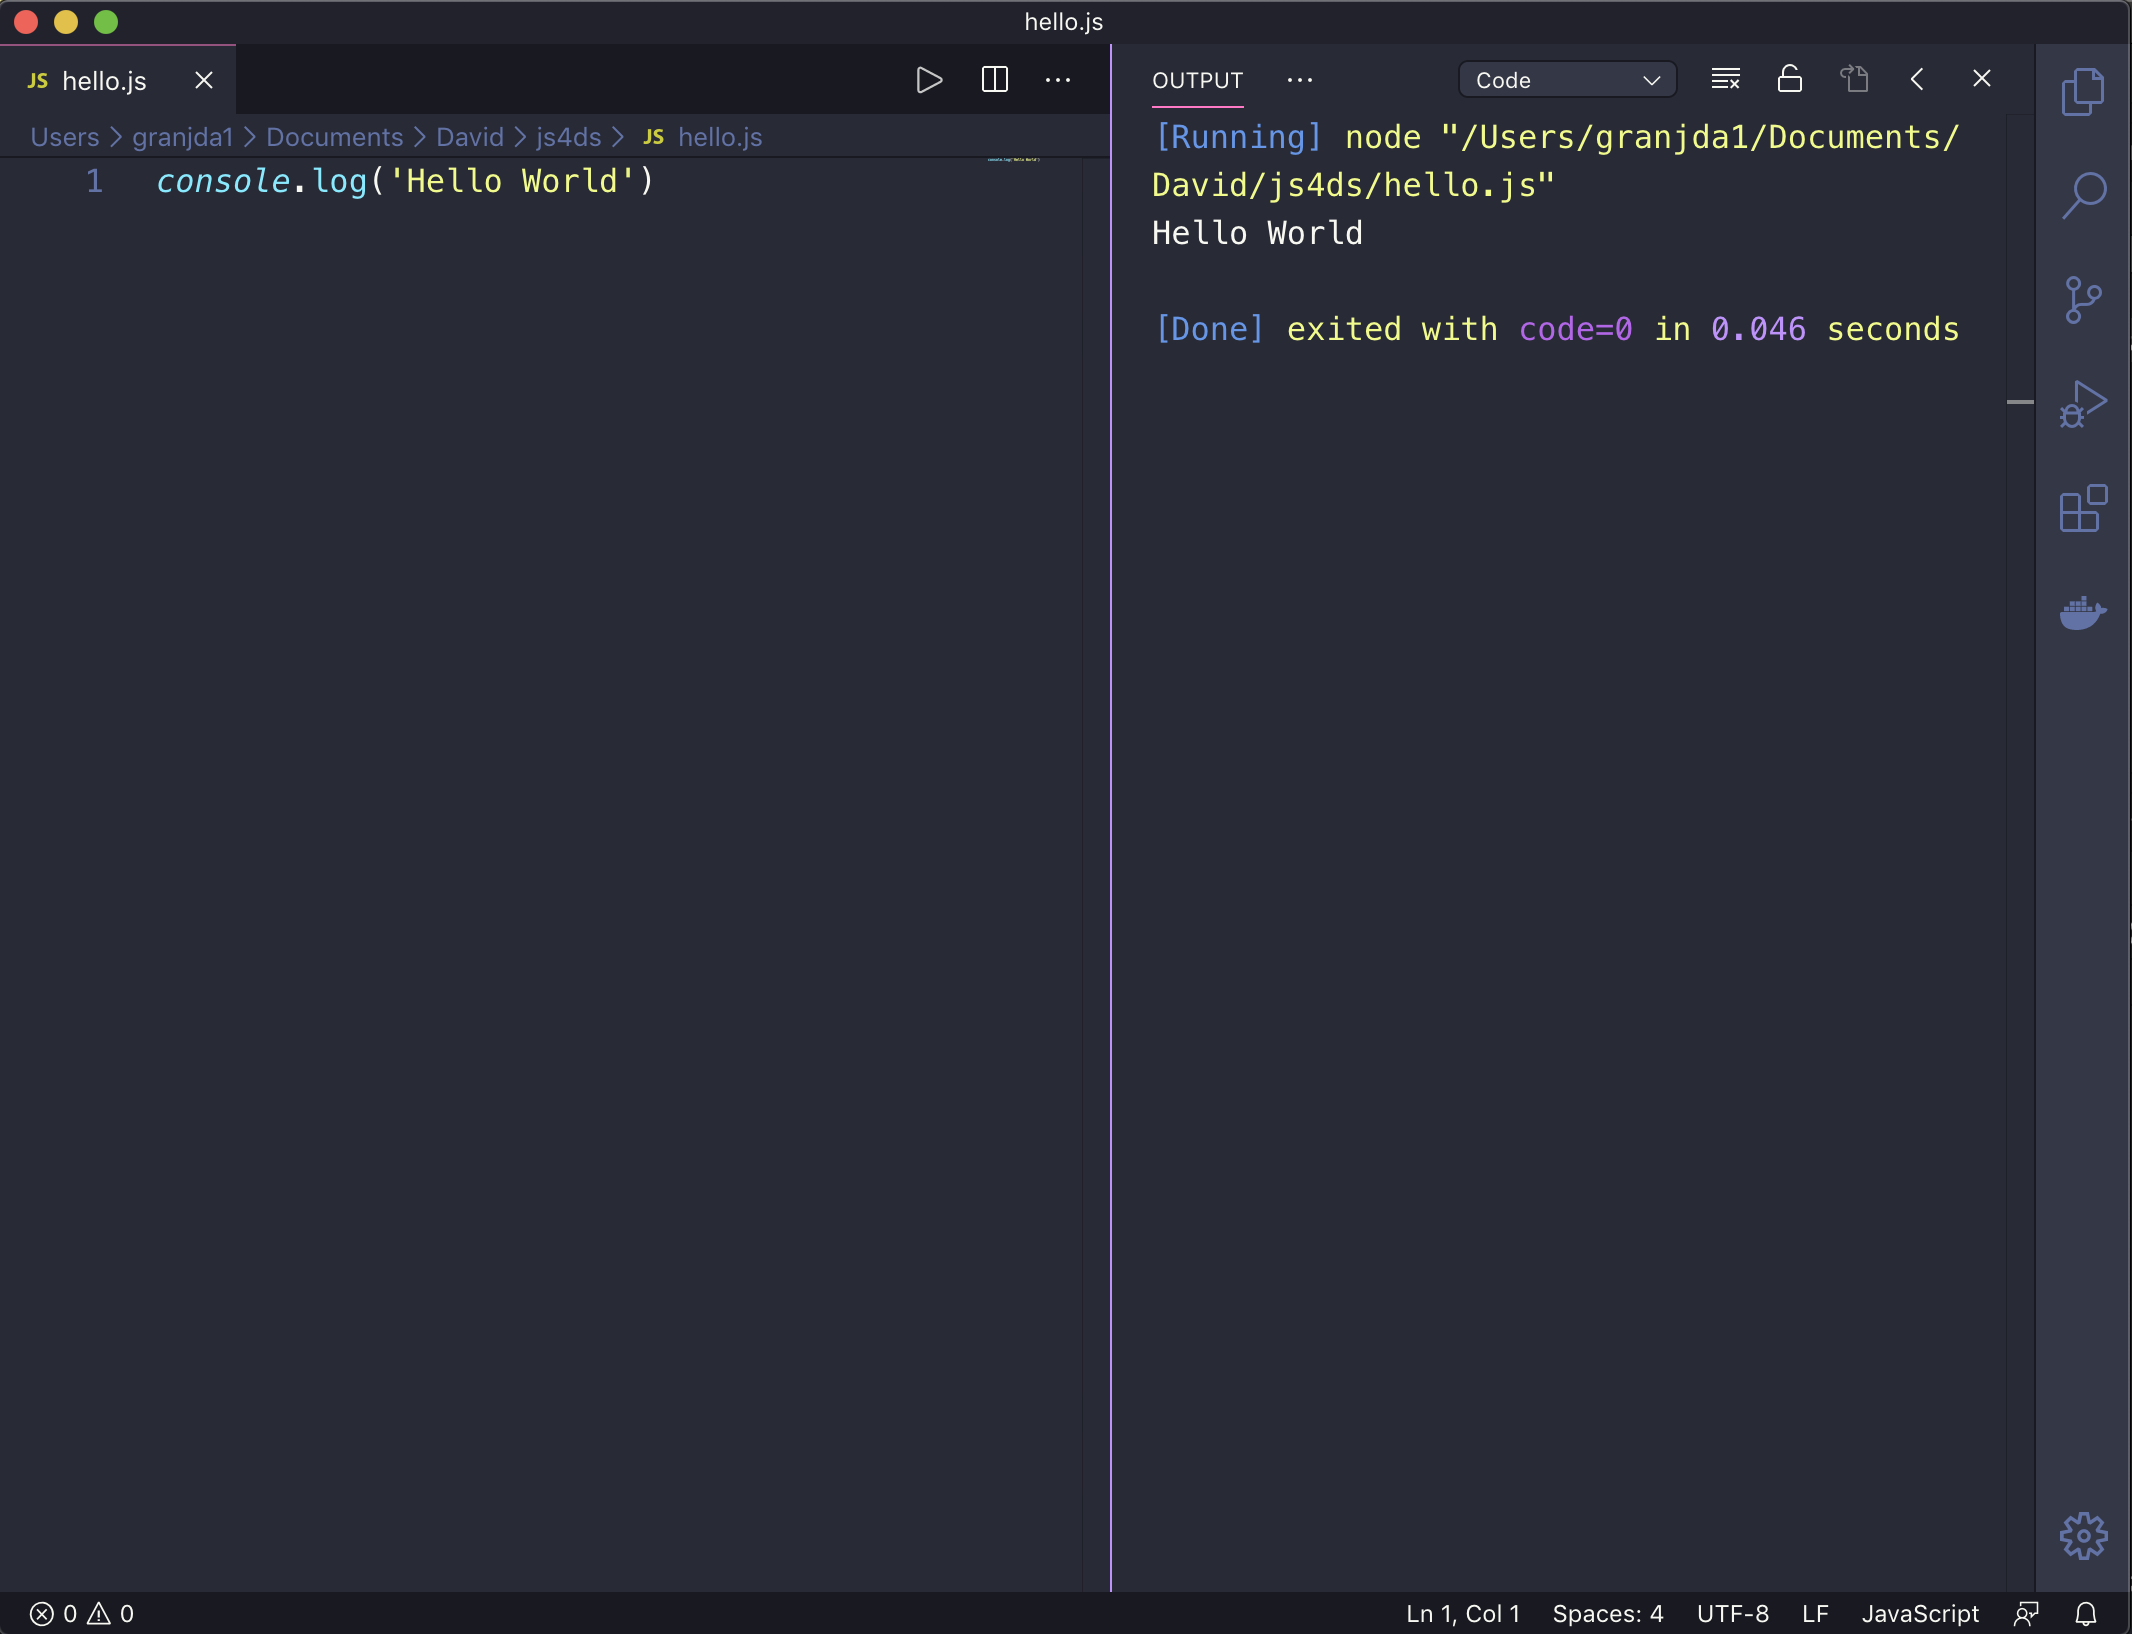
\includegraphics[width=29.61in]{images/survival-kit/script-vscode} \caption{Run JS in VSCode}\label{fig:script-vscode}
\end{figure}

In VSCode, clicking on the run arrow (top center) of Figure \ref{fig:script-vscode},
triggers the \texttt{node\ hello.js} command, which tells Node to run my script. We see the result in the right panel (code=0 means the execution is fine and we even have the compute time). To run this script in the RStudio IDE, you need to click on the terminal tab (you could also open a basic terminal) and type \texttt{node\ hello.js} (or \texttt{node\ mycustompath/hello.js} if you are not in the folder containing the script). You should see the Hello World message in the console (see Figure \ref{fig:script-rstudio}).

\begin{figure}
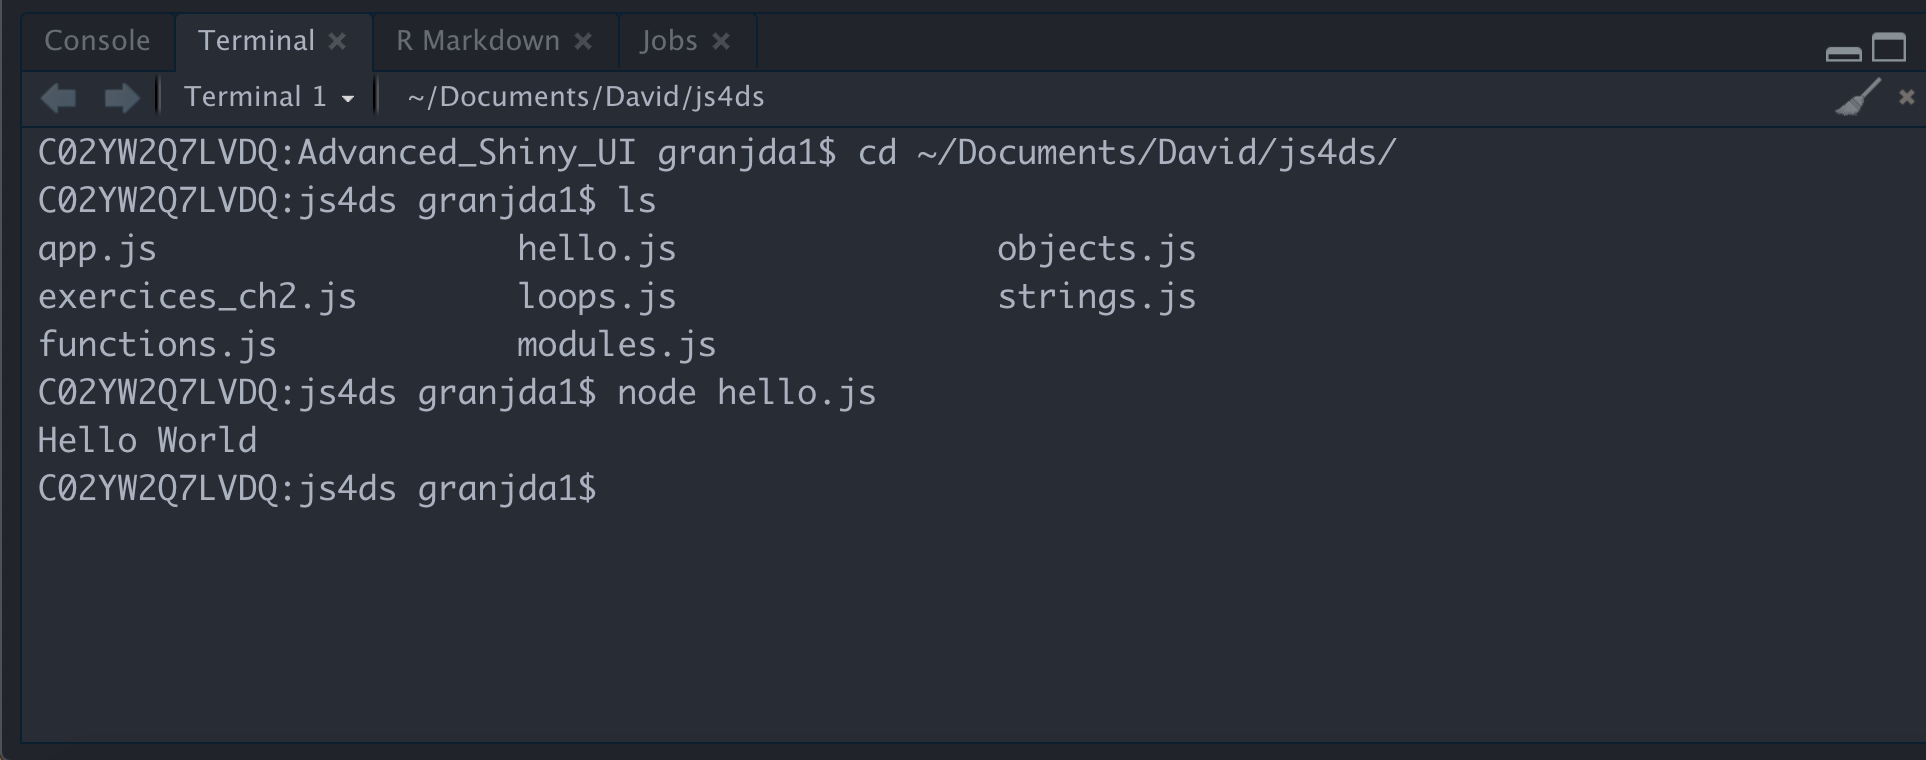
\includegraphics[width=26.75in]{images/survival-kit/script-rstudio} \caption{Run JS in a terminal}\label{fig:script-rstudio}
\end{figure}

\hypertarget{programming-with-js-basis}{%
\section{Programming with JS: basis}\label{programming-with-js-basis}}

We are now all set to introduce the basis of JS. As many languages, JS is made of variables and instructions (We saw above that instructions end by \texttt{;}).

\hypertarget{js-types}{%
\subsection{JS types}\label{js-types}}

JS defines several types:

\begin{itemize}
\tightlist
\item
  Number: does not distinguish between integers and others (in R for instance, numeric contains integers and double)
\item
  String: characters (`blabla')
\item
  Boolean: true/false
\end{itemize}

To check the type of an element, we may use the \texttt{typeof} operator (this is not a function like the \texttt{typeof} function in R).

\begin{Shaded}
\begin{Highlighting}[]
\KeywordTok{typeof} \DecValTok{1}\OperatorTok{;} \CommentTok{// number}
\KeywordTok{typeof} \StringTok{'pouic'}\OperatorTok{;} \CommentTok{// string}
\end{Highlighting}
\end{Shaded}

\hypertarget{variables}{%
\subsection{Variables}\label{variables}}

A variable is defined by:

\begin{itemize}
\tightlist
\item
  a type
\item
  a name
\item
  a value
\end{itemize}

Valid variable names:

don't use an existing name like typeof

son't start with a number (123)

don't include any space (total price)

Based on the above forbidden items, you can use the camelCase syntax to write your variables in JS. To set a variable we use \texttt{let} (there exists \texttt{var} but this is not the latest JS norm (ES6). You will see later that we still use \texttt{var} in the shiny core and many other R packages):

\begin{Shaded}
\begin{Highlighting}[]
\KeywordTok{let}\NormalTok{ myVariable }\OperatorTok{=} \StringTok{'welcome'}\OperatorTok{;}
\VariableTok{console}\NormalTok{.}\AttributeTok{log}\NormalTok{(myVariable)}\OperatorTok{;}
\end{Highlighting}
\end{Shaded}

Then we can use all mathematical operators to manipulate a variable.

\begin{Shaded}
\begin{Highlighting}[]
\KeywordTok{let}\NormalTok{ myNumber }\OperatorTok{=} \DecValTok{1}\OperatorTok{;} \CommentTok{// affectation}
\NormalTok{myNumber}\OperatorTok{--;} \CommentTok{// decrement}
\VariableTok{console}\NormalTok{.}\AttributeTok{log}\NormalTok{(myNumber)}\OperatorTok{;} \CommentTok{// print 0}
\end{Highlighting}
\end{Shaded}

List of numerical operators in JS:

+

-

*

/

\% (modulo)

++ (incrementation)

-- (decrementation)

To concatenate 2 strings, use \texttt{+}.

\hypertarget{conditions}{%
\subsection{Conditions}\label{conditions}}

Below are the operators to check conditions.

== (A equal B)

!= (A not equal to B)

\textgreater{} (\textgreater{}=)

\textless{} (\textless{}=)

AND (A AND B)

OR (A OR B)

To test conditions there exists several ways:

\begin{itemize}
\tightlist
\item
  \texttt{if\ (condition)\ \{\ console.log(\textquotesingle{}Test\ passed\textquotesingle{});\ \}}
\item
  \texttt{if\ (condition)\ \{\ instruction\ A\}\ else\ \{\ instruction\ B\ \}}
\end{itemize}

This is very common to other languages (and R for instance). Whenever a lot of possible conditions need to be evaluated, it is better to choose the \texttt{switch}.

\begin{Shaded}
\begin{Highlighting}[]
\ControlFlowTok{switch}\NormalTok{ (variable) }\OperatorTok{\{}
  \ControlFlowTok{case} \DataTypeTok{val1}\OperatorTok{:} \CommentTok{// instruction 1}
  \ControlFlowTok{break}\OperatorTok{;} \CommentTok{// don't forget the break!}
  \ControlFlowTok{case} \DataTypeTok{val2}\OperatorTok{:}  \CommentTok{// instruction 2}
  \ControlFlowTok{break}\OperatorTok{;}
  \DataTypeTok{default}\OperatorTok{:} \CommentTok{// when none of val1 and val2 are satisfied}
\OperatorTok{\}}
\end{Highlighting}
\end{Shaded}

\hypertarget{iterations}{%
\subsection{Iterations}\label{iterations}}

Iterations allow to repeat an instruction or a set of instructions multiple times.

\hypertarget{for-loops}{%
\subsubsection{For loops}\label{for-loops}}

The for loop has multiple ways to be used. Below is the most classic. We start by defining the index (variable). We then set an upper bound and we finish by incrementing the index value. We execute the instruction between curly braces.

\begin{Shaded}
\begin{Highlighting}[]
\KeywordTok{const}\NormalTok{ max }\OperatorTok{=} \DecValTok{10}\OperatorTok{;} \CommentTok{// we never mentionned constants before. This is the way to call them}
\ControlFlowTok{for}\NormalTok{ (}\KeywordTok{let}\NormalTok{ i }\OperatorTok{=} \DecValTok{0}\OperatorTok{;}\NormalTok{ i }\OperatorTok{<=}\NormalTok{ max}\OperatorTok{;}\NormalTok{ i}\OperatorTok{++}\NormalTok{) }\OperatorTok{\{}
  \VariableTok{console}\NormalTok{.}\AttributeTok{log}\NormalTok{(i)}\OperatorTok{;} \CommentTok{// this will print i 10 times}
\OperatorTok{\}}
\end{Highlighting}
\end{Shaded}

Contrary to R, JavaScript index starts from 0 (not from 1)! This is good to keep in mind when we will mix both R and JS.

Below is another way to create a for loop:

\begin{Shaded}
\begin{Highlighting}[]
\KeywordTok{let}\NormalTok{ samples }\OperatorTok{=}\NormalTok{ [}\StringTok{'blabla'}\OperatorTok{,} \DecValTok{1}\OperatorTok{,} \KeywordTok{null}\NormalTok{]}\OperatorTok{;} \CommentTok{// this is an array!}
\ControlFlowTok{for}\NormalTok{ (}\KeywordTok{let}\NormalTok{ sample of samples) }\OperatorTok{\{}
 \VariableTok{console}\NormalTok{.}\AttributeTok{log}\NormalTok{(sample)}\OperatorTok{;}
\OperatorTok{\}}
\end{Highlighting}
\end{Shaded}

What is the best \texttt{for} loop? The answer is: it depends on the situation! Actually, there even exists other ways (replace of by in and you get the indexes of the array, like the with the first code, but this is really \href{https://hacks.mozilla.org/2015/04/es6-in-depth-iterators-and-the-for-of-loop/}{not recommended}).

\hypertarget{other-iterations-while}{%
\subsubsection{Other iterations: while}\label{other-iterations-while}}

We will clearly never use them in this book but this is good to know.

\begin{Shaded}
\begin{Highlighting}[]
\KeywordTok{const}\NormalTok{ h }\OperatorTok{=} \DecValTok{3}\OperatorTok{;}\NormalTok{ i }\OperatorTok{=} \DecValTok{0}\OperatorTok{;}
\ControlFlowTok{while}\NormalTok{ (i }\OperatorTok{<=}\NormalTok{ h) }\OperatorTok{\{}
  \VariableTok{console}\NormalTok{.}\AttributeTok{log}\NormalTok{(i)}\OperatorTok{;}
\NormalTok{  i}\OperatorTok{++;} \CommentTok{// we need to increment to avoid infinite loop}
\OperatorTok{\}}
\end{Highlighting}
\end{Shaded}

\hypertarget{objects}{%
\subsection{Objects}\label{objects}}

JavaScript is an object oriented programming language (like Python). An object is defined by:

\begin{itemize}
\tightlist
\item
  a type
\item
  some properties
\item
  some methods (to manipulate properties)
\end{itemize}

Let's define our first object below:

\begin{Shaded}
\begin{Highlighting}[]
\KeywordTok{const}\NormalTok{ me }\OperatorTok{=} \OperatorTok{\{}
  \DataTypeTok{name }\OperatorTok{:} \StringTok{'Divad'}\OperatorTok{,}
  \DataTypeTok{age }\OperatorTok{:} \DecValTok{29}\OperatorTok{,}
  \DataTypeTok{music }\OperatorTok{:} \StringTok{''}\OperatorTok{,}
  \DataTypeTok{printName}\OperatorTok{:} \KeywordTok{function}\NormalTok{() }\OperatorTok{\{}
    \VariableTok{console}\NormalTok{.}\AttributeTok{log}\NormalTok{(}\VerbatimStringTok{`I am }\SpecialCharTok{$\{}\KeywordTok{this}\NormalTok{.}\AttributeTok{name}\SpecialCharTok{\}}\VerbatimStringTok{`}\NormalTok{)}\OperatorTok{;}
  \OperatorTok{\}}
\OperatorTok{\}}

\VariableTok{console}\NormalTok{.}\AttributeTok{log}\NormalTok{(}\VariableTok{JSON}\NormalTok{.}\AttributeTok{stringify}\NormalTok{(me))}\OperatorTok{;} \CommentTok{// print a human readable object.}
  
\VariableTok{console}\NormalTok{.}\AttributeTok{log}\NormalTok{(}\VariableTok{me}\NormalTok{.}\AttributeTok{name}\NormalTok{)}\OperatorTok{;}
\VariableTok{console}\NormalTok{.}\AttributeTok{log}\NormalTok{(}\VariableTok{me}\NormalTok{.}\AttributeTok{age}\NormalTok{)}\OperatorTok{;}
\VariableTok{console}\NormalTok{.}\AttributeTok{log}\NormalTok{(}\VariableTok{me}\NormalTok{.}\AttributeTok{music}\NormalTok{)}\OperatorTok{;}
\CommentTok{// don't repeat yourself!!!}
\ControlFlowTok{for}\NormalTok{ (}\KeywordTok{let}\NormalTok{ key }\KeywordTok{in}\NormalTok{ me) }\OperatorTok{\{} \CommentTok{// here is it ok to use `in`}
 \VariableTok{console}\NormalTok{.}\AttributeTok{log}\NormalTok{(}\VerbatimStringTok{`me[}\SpecialCharTok{$\{}\NormalTok{key}\SpecialCharTok{\}}\VerbatimStringTok{] is }\SpecialCharTok{$\{}\NormalTok{me[key]}\SpecialCharTok{\}}\VerbatimStringTok{`}\NormalTok{)}\OperatorTok{;}
\OperatorTok{\}}

\VariableTok{me}\NormalTok{.}\AttributeTok{printName}\NormalTok{()}\OperatorTok{;}
\end{Highlighting}
\end{Shaded}

Some comments on the above code:

\begin{itemize}
\tightlist
\item
  to access an object propertie, we use \texttt{object.propertie}
\item
  to print a human readable version of the object \texttt{JSON.stringify} will do the job
\item
  we introduced string interpolation with \texttt{\$\{*\}}. \texttt{*} may be any valid expression.
\item
  methods are accessed like properties (we may also pass parameters). We use \texttt{this} to refer to the object itself. Take note, we will see it a lot!
\end{itemize}

In JavaScript, we can find already predefined objects to interact with arrays, dates.

\hypertarget{arrays}{%
\subsubsection{Arrays}\label{arrays}}

An array is a structure allowing to store informations for instance

\begin{Shaded}
\begin{Highlighting}[]
\KeywordTok{let}\NormalTok{ table }\OperatorTok{=}\NormalTok{ [}\DecValTok{1}\OperatorTok{,} \StringTok{'plop'}\NormalTok{]}\OperatorTok{;}
\VariableTok{console}\NormalTok{.}\AttributeTok{log}\NormalTok{(table)}\OperatorTok{;}
\end{Highlighting}
\end{Shaded}

Array may be nested

\begin{Shaded}
\begin{Highlighting}[]
\KeywordTok{let}\NormalTok{ nested }\OperatorTok{=}\NormalTok{ [}\DecValTok{1}\OperatorTok{,}\NormalTok{ [}\StringTok{'a'}\OperatorTok{,}\NormalTok{ [}\DecValTok{1}\OperatorTok{,} \DecValTok{2}\OperatorTok{,} \DecValTok{3}\NormalTok{]]}\OperatorTok{,} \StringTok{'plop'}\NormalTok{]}\OperatorTok{;}
\VariableTok{console}\NormalTok{.}\AttributeTok{log}\NormalTok{(nested)}\OperatorTok{;}
\end{Highlighting}
\end{Shaded}

In arrays, elements may be accessed by their index, but as mentionned before, the first index is 0 (not 1 like in R). A convenient way to print all arrays's elements is to use an iteration:

\begin{Shaded}
\begin{Highlighting}[]
\KeywordTok{let}\NormalTok{ nested }\OperatorTok{=}\NormalTok{ [}\DecValTok{1}\OperatorTok{,}\NormalTok{ [}\StringTok{'a'}\OperatorTok{,}\NormalTok{ [}\DecValTok{1}\OperatorTok{,} \DecValTok{2}\OperatorTok{,} \DecValTok{3}\NormalTok{]]}\OperatorTok{,} \StringTok{'plop'}\NormalTok{]}\OperatorTok{;}
\ControlFlowTok{for}\NormalTok{ (}\KeywordTok{let}\NormalTok{ i of nested) }\OperatorTok{\{}
  \VariableTok{console}\NormalTok{.}\AttributeTok{log}\NormalTok{(i)}\OperatorTok{;}
\OperatorTok{\}}

\CommentTok{// or with the classic approach}
\ControlFlowTok{for}\NormalTok{ (}\KeywordTok{let}\NormalTok{ i }\OperatorTok{=} \DecValTok{0}\OperatorTok{;}\NormalTok{ i }\OperatorTok{<} \VariableTok{nested}\NormalTok{.}\AttributeTok{length}\OperatorTok{;}\NormalTok{ i}\OperatorTok{++}\NormalTok{) }\OperatorTok{\{}
  \VariableTok{console}\NormalTok{.}\AttributeTok{log}\NormalTok{(nested[i])}\OperatorTok{;}
\OperatorTok{\}}
\end{Highlighting}
\end{Shaded}

Note that the \texttt{length} method returns the size of an array and is very convenient in for loops. Below is a table referencing the principal methods for arrays (we will use some of them later)

\begin{longtable}[]{@{}cc@{}}
\toprule
Method/Property & Description\tabularnewline
\midrule
\endhead
length & Return the number of elements in an array\tabularnewline
Join(string separator) & Transform an array in a string\tabularnewline
concat(array1, array2) & Assemble 2 arrays\tabularnewline
pop() & Remove the last element of an array\tabularnewline
shift() & Remove the first element of an array\tabularnewline
unshift(el1, el2, \ldots{}) & Insert elements at the beginning of an array\tabularnewline
push(el1, el2, \ldots{}) & Add extra elements at the end of an array\tabularnewline
sort() & Sort array elements by increasing value of alphabetical order\tabularnewline
reverse() & Symetric of sort()\tabularnewline
\bottomrule
\end{longtable}

Quite honestly, we will only use \texttt{push} and \texttt{length} in the next chapters.

\hypertarget{strings}{%
\subsubsection{Strings}\label{strings}}

Below are the main methods related to the String object (character in R)

\begin{longtable}[]{@{}cc@{}}
\toprule
Method/Property/Operator & Description\tabularnewline
\midrule
\endhead
+ (operator) & String concatenation\tabularnewline
length & String length\tabularnewline
indexOf() & Gives the position of the character following the input string\tabularnewline
toLowerCase() & Put the string in small letters\tabularnewline
toUpperCase() & Put the string in capital letters\tabularnewline
\bottomrule
\end{longtable}

\hypertarget{math}{%
\subsubsection{Math}\label{math}}

Below we mention some useful methods to handle mathematical objects

\begin{longtable}[]{@{}cc@{}}
\toprule
Method & Description\tabularnewline
\midrule
\endhead
parseInt() & Convert a string to integer\tabularnewline
parseFloat() & Conversion to floating number\tabularnewline
\bottomrule
\end{longtable}

All classic functions like \texttt{sqrt}, trigonometric functions are of course available. We call them with the \texttt{Math.*} prefix.

\hypertarget{functions}{%
\subsection{Functions}\label{functions}}

Functions are useful to wrap a succession of instructions to accomplish a given task. Defining functions allows programmers to save time (less copy and paste, less search and replace), do less errors and share code more easily. In modern JavaScript (ES6), functions are defined as follows:

\begin{Shaded}
\begin{Highlighting}[]
\KeywordTok{const}\NormalTok{ a }\OperatorTok{=} \DecValTok{1}\OperatorTok{;}
\KeywordTok{const}\NormalTok{ fun }\OperatorTok{=}\NormalTok{ (parm1}\OperatorTok{,}\NormalTok{ parm2) }\OperatorTok{=>} \OperatorTok{\{}
  \VariableTok{console}\NormalTok{.}\AttributeTok{log}\NormalTok{(a)}\OperatorTok{;}
  \KeywordTok{let}\NormalTok{ p }\OperatorTok{=} \DecValTok{3}\OperatorTok{;}
  \ControlFlowTok{return} \VariableTok{Math}\NormalTok{.}\AttributeTok{max}\NormalTok{(parm1}\OperatorTok{,}\NormalTok{ parm2)}\OperatorTok{;} \CommentTok{// I use the Math object that contains the max method}
\OperatorTok{\}}
\KeywordTok{let}\NormalTok{ res }\OperatorTok{=} \AttributeTok{fun}\NormalTok{(}\DecValTok{1}\OperatorTok{,} \DecValTok{2}\NormalTok{)}\OperatorTok{;}
\VariableTok{console}\NormalTok{.}\AttributeTok{log}\NormalTok{(res)}\OperatorTok{;} \CommentTok{// prints a and 2. a global}
\VariableTok{console}\NormalTok{.}\AttributeTok{log}\NormalTok{(p)}\OperatorTok{;} \CommentTok{// fails because p was defined inside the function}
\end{Highlighting}
\end{Shaded}

This functions computes the maximum of 2 provided numbers. Some comments about scoping rules: variables defined inside the function are available for the function but not outside. The function may use global variables defined outside of it.

\hypertarget{export-functions-about-modules}{%
\subsubsection{Export functions: about modules}\label{export-functions-about-modules}}

What happens if you wrote 100 functions and you would like to reuse some of them in different scripts? To prevent copy and pasting, we will introduce modules. Let's save the below function in a script \texttt{utils.js}:

\begin{Shaded}
\begin{Highlighting}[]
\KeywordTok{const}\NormalTok{ findMax }\OperatorTok{=}\NormalTok{ (parm1}\OperatorTok{,}\NormalTok{ parm2) }\OperatorTok{=>} \OperatorTok{\{}
  \ControlFlowTok{return} \VariableTok{Math}\NormalTok{.}\AttributeTok{max}\NormalTok{(parm1}\OperatorTok{,}\NormalTok{ parm2)}\OperatorTok{;} \CommentTok{// I use the Math object that contains the max method}
\OperatorTok{\}}

\VariableTok{module}\NormalTok{.}\AttributeTok{exports} \OperatorTok{=} \OperatorTok{\{}
\NormalTok{  findMax }\OperatorTok{=}\NormalTok{ findMax}
\OperatorTok{\}}
\end{Highlighting}
\end{Shaded}

Now, if we create a \texttt{test.js} script in the same folder and want to use \texttt{findMax}, we need to import the corresponding module:

\begin{Shaded}
\begin{Highlighting}[]
\KeywordTok{const} \OperatorTok{\{}\NormalTok{findMax}\OperatorTok{\}} \OperatorTok{=} \AttributeTok{require}\NormalTok{(}\StringTok{'./utils.js'}\NormalTok{)}\OperatorTok{;}
\AttributeTok{findMax}\NormalTok{(}\DecValTok{1}\OperatorTok{,} \DecValTok{2}\NormalTok{)}\OperatorTok{;} \CommentTok{// prints 2}
\end{Highlighting}
\end{Shaded}

In the next chapters, we will see that some of the underlying JS code to build custom shiny inputs share the same utils functions. Therefore, introducing modules is necessary.

\hypertarget{event-listeners}{%
\subsection{Event listeners}\label{event-listeners}}

When you explore a web application, clicking on a button usually triggers something like a computation, a modal or an alert. How does this work?
In JavaScript, interactivity plays a critical role. Indeed, you want the web application to react to user inputs like mouse clicks, keyboard events. Below we introduce DOM events.

Let's consider a basic HTML button.

\begin{Shaded}
\begin{Highlighting}[]
\KeywordTok{<button}\OtherTok{ id=}\StringTok{"mybutton"}\KeywordTok{>}\NormalTok{Go!}\KeywordTok{</button>}
\end{Highlighting}
\end{Shaded}

On the JavaScript side, we first capture the button element using its id selector (\texttt{getElementById}).

\begin{Shaded}
\begin{Highlighting}[]
\KeywordTok{const}\NormalTok{ btn }\OperatorTok{=} \VariableTok{document}\NormalTok{.}\AttributeTok{getElementById}\NormalTok{(}\StringTok{'mybutton'}\NormalTok{)}\OperatorTok{;}
\end{Highlighting}
\end{Shaded}

We then apply the \texttt{addEventListener} method. In short, an event listener is a program that triggers when a given event occurs (we can add multiple event listeners per HTML element). It takes 2 main parameters:

\begin{itemize}
\tightlist
\item
  the event: click, change, mouseover, \ldots{}
\item
  the function to call
\end{itemize}

\begin{Shaded}
\begin{Highlighting}[]
\VariableTok{btn}\NormalTok{.}\AttributeTok{addEventListener}\NormalTok{(}\StringTok{'click'}\OperatorTok{,} \KeywordTok{function}\NormalTok{() }\OperatorTok{\{}
  \AttributeTok{alert}\NormalTok{(}\StringTok{'Thanks!'}\NormalTok{)}\OperatorTok{;}
\OperatorTok{\}}\NormalTok{)}\OperatorTok{;}
\end{Highlighting}
\end{Shaded}

We could compare the JavaScript events to Shiny observeEvent in which we are listenning to a specific user input.

\hypertarget{jquery}{%
\section{jQuery}\label{jquery}}

\hypertarget{introduction-1}{%
\subsection{Introduction}\label{introduction-1}}

\href{https://jquery.com}{jQuery} is a famous JavaScript library providing a user friendly interface to manipulate the DOM and is present in almost all actual websites. It is slighly easier (understand more convenient to use) than vanilla JS, even though web developers tend to avoid it to go back to vanilla JS (Bootstrap 5, the next iteration of Bootstrap will not rely on jQuery anymore). To use jQuery in a webpage, we must include its code either by dowloading the code and putting the minified JS file in our HTML or setting a link to a CDN.

\begin{Shaded}
\begin{Highlighting}[]
\DataTypeTok{<!doctype }\NormalTok{html}\DataTypeTok{>}
\KeywordTok{<html}\OtherTok{ lang=}\StringTok{"en"}\KeywordTok{>}
\KeywordTok{<head>}
  \KeywordTok{<meta}\OtherTok{ charset=}\StringTok{"utf-8"}\KeywordTok{>}
  \KeywordTok{<title>}\NormalTok{Including jQuery}\KeywordTok{</title>}
  \CommentTok{<!-- How to include jQuery -->}
  \KeywordTok{<script}\OtherTok{ src=}\StringTok{"https://code.jquery.com/jquery-3.5.0.js"}\KeywordTok{></script>}
\KeywordTok{</head>}
\KeywordTok{<body>}
 
\KeywordTok{<p>}\NormalTok{Hello World}\KeywordTok{</p>}

 
\KeywordTok{<script>}
\AttributeTok{$}\NormalTok{(}\StringTok{'p'}\NormalTok{).}\AttributeTok{css}\NormalTok{(}\StringTok{'color'}\OperatorTok{,} \StringTok{'red'}\NormalTok{)}\OperatorTok{;}
\KeywordTok{</script>}
 
\KeywordTok{</body>}
\KeywordTok{</html>}
\end{Highlighting}
\end{Shaded}

\hypertarget{syntax}{%
\subsection{Syntax}\label{syntax}}

Below is a minimal jQuery code representing its philosophy (``write less, do more.''):

\begin{Shaded}
\begin{Highlighting}[]
\AttributeTok{$}\NormalTok{(selector).}\AttributeTok{action}\NormalTok{()}\OperatorTok{;}
\end{Highlighting}
\end{Shaded}

The selector slot stands for any jQuery selector like class, id, element, {[}attribute{]}, :input (will select all input elements) and many \href{https://www.w3schools.com/jquery/jquery_ref_selectors.asp}{more}. As a reminder, let's consider the following example:

\begin{Shaded}
\begin{Highlighting}[]
\KeywordTok{<p}\OtherTok{ class=}\StringTok{"text"}\KeywordTok{>}\NormalTok{Hello World}\KeywordTok{</p>}
\end{Highlighting}
\end{Shaded}

To select and interact with this element, we use JavaScript and jQuery:

\begin{Shaded}
\begin{Highlighting}[]
\KeywordTok{let}\NormalTok{ inner }\OperatorTok{=} \VariableTok{document}\NormalTok{.}\AttributeTok{getElementsByClassName}\NormalTok{(}\StringTok{'text'}\NormalTok{).}\AttributeTok{innerHTML}\OperatorTok{;} \CommentTok{// vanilla JS}
\KeywordTok{let}\NormalTok{ inner }\OperatorTok{=} \AttributeTok{$}\NormalTok{(}\StringTok{'.text'}\NormalTok{).}\AttributeTok{html}\NormalTok{()}\OperatorTok{;} \CommentTok{// jQuery}
\end{Highlighting}
\end{Shaded}

This is of course possible to chain selectors

\begin{Shaded}
\begin{Highlighting}[]
\KeywordTok{<ul}\OtherTok{ class=}\StringTok{"list"}\KeywordTok{>}
  \KeywordTok{<li}\OtherTok{ class=}\StringTok{"item"}\KeywordTok{>}\NormalTok{1}\KeywordTok{</li>}
  \KeywordTok{<li}\OtherTok{ class=}\StringTok{"item"}\KeywordTok{>}\NormalTok{2}\KeywordTok{</li>}
  \KeywordTok{<li}\OtherTok{ class=}\StringTok{"item"}\KeywordTok{>}\NormalTok{3}\KeywordTok{</li>}
  \KeywordTok{<li}\OtherTok{ class=}\StringTok{"item"}\OtherTok{ id=}\StringTok{"precious-item"}\KeywordTok{>}\NormalTok{4}\KeywordTok{</li>}
\KeywordTok{</ul>}

\KeywordTok{<ul}\OtherTok{ class=}\StringTok{"list"}\OtherTok{ id=}\StringTok{"list2"}\KeywordTok{>}
  \KeywordTok{<li}\OtherTok{ class=}\StringTok{"item"}\KeywordTok{>}\NormalTok{1}\KeywordTok{</li>}
  \KeywordTok{<li}\OtherTok{ class=}\StringTok{"item"}\KeywordTok{>}\NormalTok{2}\KeywordTok{</li>}
  \KeywordTok{<li}\OtherTok{ class=}\StringTok{"item"}\KeywordTok{>}\NormalTok{3}\KeywordTok{</li>}
  \KeywordTok{<li}\OtherTok{ class=}\StringTok{"item"}\KeywordTok{>}\NormalTok{4}\KeywordTok{</li>}
\KeywordTok{</ul>}
\end{Highlighting}
\end{Shaded}

\begin{Shaded}
\begin{Highlighting}[]
\KeywordTok{let}\NormalTok{ items }\OperatorTok{=} \AttributeTok{$}\NormalTok{(}\StringTok{'.list .item'}\NormalTok{)}\OperatorTok{;} \CommentTok{// will return an array containing 8 li tags}
\KeywordTok{let}\NormalTok{ otherItems }\OperatorTok{=} \AttributeTok{$}\NormalTok{(}\StringTok{'#list2 .item'}\NormalTok{)}\OperatorTok{;} \CommentTok{// will select only li tags from the second ul element}
\KeywordTok{let}\NormalTok{ lists }\OperatorTok{=} \AttributeTok{$}\NormalTok{(}\StringTok{'ul'}\NormalTok{)}\OperatorTok{;} \CommentTok{// will return an array with 2 ul elements}
\KeywordTok{let}\NormalTok{ firstItem }\OperatorTok{=} \AttributeTok{$}\NormalTok{(}\StringTok{'#list2:first-child'}\NormalTok{)}\OperatorTok{;} \CommentTok{// will return the first li element of the second ul.}
\end{Highlighting}
\end{Shaded}

jQuery is obviously simpler than pure JavaScript.

\hypertarget{useful-functions}{%
\subsection{Useful functions}\label{useful-functions}}

There exist filtering functions dedicated to simplify item \href{https://api.jquery.com/category/traversing/}{selection}. We gathered the one mostly used in Shiny below.

\hypertarget{travel-in-the-dom}{%
\subsubsection{Travel in the DOM}\label{travel-in-the-dom}}

\begin{longtable}[]{@{}cc@{}}
\toprule
\begin{minipage}[b]{0.42\columnwidth}\centering
Method\strut
\end{minipage} & \begin{minipage}[b]{0.52\columnwidth}\centering
Description\strut
\end{minipage}\tabularnewline
\midrule
\endhead
\begin{minipage}[t]{0.42\columnwidth}\centering
children()\strut
\end{minipage} & \begin{minipage}[t]{0.52\columnwidth}\centering
Get the children of each element passed in the selector (important: only travels a single level down the DOM tree)\strut
\end{minipage}\tabularnewline
\begin{minipage}[t]{0.42\columnwidth}\centering
first()\strut
\end{minipage} & \begin{minipage}[t]{0.52\columnwidth}\centering
Given an list of elements, select the first item\strut
\end{minipage}\tabularnewline
\begin{minipage}[t]{0.42\columnwidth}\centering
last()\strut
\end{minipage} & \begin{minipage}[t]{0.52\columnwidth}\centering
Given an list of elements, select the last item\strut
\end{minipage}\tabularnewline
\begin{minipage}[t]{0.42\columnwidth}\centering
find()\strut
\end{minipage} & \begin{minipage}[t]{0.52\columnwidth}\centering
Look for a descendant of the selected element(s) that could be multiple levels down in the DOM\strut
\end{minipage}\tabularnewline
\begin{minipage}[t]{0.42\columnwidth}\centering
closest()\strut
\end{minipage} & \begin{minipage}[t]{0.52\columnwidth}\centering
Returns the first ancestor matching the condition (travels up in the DOM)\strut
\end{minipage}\tabularnewline
\begin{minipage}[t]{0.42\columnwidth}\centering
filter()\strut
\end{minipage} & \begin{minipage}[t]{0.52\columnwidth}\centering
Fine tune element selection by applying a filter. Only return element for which the condition is true\strut
\end{minipage}\tabularnewline
\begin{minipage}[t]{0.42\columnwidth}\centering
siblings()\strut
\end{minipage} & \begin{minipage}[t]{0.52\columnwidth}\centering
Get all siblings of the selected element(s)\strut
\end{minipage}\tabularnewline
\begin{minipage}[t]{0.42\columnwidth}\centering
next()\strut
\end{minipage} & \begin{minipage}[t]{0.52\columnwidth}\centering
Get the immediately following sibling\strut
\end{minipage}\tabularnewline
\begin{minipage}[t]{0.42\columnwidth}\centering
prev()\strut
\end{minipage} & \begin{minipage}[t]{0.52\columnwidth}\centering
Get the immediately preceding sibling\strut
\end{minipage}\tabularnewline
\begin{minipage}[t]{0.42\columnwidth}\centering
not()\strut
\end{minipage} & \begin{minipage}[t]{0.52\columnwidth}\centering
Given an existing set of selected elements, remove element(s) that match the given condition\strut
\end{minipage}\tabularnewline
\bottomrule
\end{longtable}

\hypertarget{manipulate-tags}{%
\subsubsection{Manipulate tags}\label{manipulate-tags}}

Below is a list of the main jQuery \href{https://api.jquery.com/category/manipulation/}{methods} to manipulate tags (adding class, css property\ldots{})

\begin{longtable}[]{@{}cc@{}}
\toprule
\begin{minipage}[b]{0.42\columnwidth}\centering
Method\strut
\end{minipage} & \begin{minipage}[b]{0.52\columnwidth}\centering
Description\strut
\end{minipage}\tabularnewline
\midrule
\endhead
\begin{minipage}[t]{0.42\columnwidth}\centering
addClass()\strut
\end{minipage} & \begin{minipage}[t]{0.52\columnwidth}\centering
Add class or multiple classes to the set of matched elements\strut
\end{minipage}\tabularnewline
\begin{minipage}[t]{0.42\columnwidth}\centering
hasClass()\strut
\end{minipage} & \begin{minipage}[t]{0.52\columnwidth}\centering
Check if the matched element(s) have a given class\strut
\end{minipage}\tabularnewline
\begin{minipage}[t]{0.42\columnwidth}\centering
removeClass()\strut
\end{minipage} & \begin{minipage}[t]{0.52\columnwidth}\centering
Remove class or multiple classes to the set of matched elements\strut
\end{minipage}\tabularnewline
\begin{minipage}[t]{0.42\columnwidth}\centering
attr()\strut
\end{minipage} & \begin{minipage}[t]{0.52\columnwidth}\centering
Get or set the value of a specific attribute\strut
\end{minipage}\tabularnewline
\begin{minipage}[t]{0.42\columnwidth}\centering
after()\strut
\end{minipage} & \begin{minipage}[t]{0.52\columnwidth}\centering
Insert content after\strut
\end{minipage}\tabularnewline
\begin{minipage}[t]{0.42\columnwidth}\centering
before ()\strut
\end{minipage} & \begin{minipage}[t]{0.52\columnwidth}\centering
Insert content before\strut
\end{minipage}\tabularnewline
\begin{minipage}[t]{0.42\columnwidth}\centering
css()\strut
\end{minipage} & \begin{minipage}[t]{0.52\columnwidth}\centering
Get or set a css property\strut
\end{minipage}\tabularnewline
\begin{minipage}[t]{0.42\columnwidth}\centering
remove()\strut
\end{minipage} & \begin{minipage}[t]{0.52\columnwidth}\centering
Remove element(s) from the DOM\strut
\end{minipage}\tabularnewline
\begin{minipage}[t]{0.42\columnwidth}\centering
val()\strut
\end{minipage} & \begin{minipage}[t]{0.52\columnwidth}\centering
Get the current value of the matched element(s)\strut
\end{minipage}\tabularnewline
\bottomrule
\end{longtable}

TO DO: add more methods

\hypertarget{chaining-jquery-methods}{%
\subsection{Chaining jQuery methods}\label{chaining-jquery-methods}}

A lot of jQuery methods may be chained, that is like pipe operations in R.

\begin{Shaded}
\begin{Highlighting}[]
\KeywordTok{<ul>}
  \KeywordTok{<li>}\NormalTok{Item 1}\KeywordTok{</li>}
  \KeywordTok{<li>}\NormalTok{Item 2}\KeywordTok{</li>}
  \KeywordTok{<li>}\NormalTok{Item 3}\KeywordTok{</li>}
  \KeywordTok{<li>}\NormalTok{Item 4}\KeywordTok{</li>}
  \KeywordTok{<li>}\NormalTok{Item 5}\KeywordTok{</li>}
\KeywordTok{</ul>}
\end{Highlighting}
\end{Shaded}

We end the chain by \texttt{;} and each step is indent by 2 spaces in the right direction.

\begin{Shaded}
\begin{Highlighting}[]
\AttributeTok{$}\NormalTok{(}\StringTok{'ul'}\NormalTok{)}
\NormalTok{  .}\AttributeTok{first}\NormalTok{()}
\NormalTok{  .}\AttributeTok{css}\NormalTok{(}\StringTok{'color'}\OperatorTok{,} \StringTok{'green'}\NormalTok{) }\CommentTok{// add some style with css}
\NormalTok{  .}\AttributeTok{attr}\NormalTok{(}\StringTok{'id'}\OperatorTok{,} \StringTok{'myAwesomeItem'}\NormalTok{) }\CommentTok{// add an id attribute}
\NormalTok{  .}\AttributeTok{addClass}\NormalTok{(}\StringTok{'amazing-ul'}\NormalTok{)}\OperatorTok{;}
\end{Highlighting}
\end{Shaded}

\hypertarget{iterations-1}{%
\subsection{Iterations}\label{iterations-1}}

Like in vanilla JavaScript, it is possible to do iterations in jQuery. Let's consider the following HTML elements.

\begin{Shaded}
\begin{Highlighting}[]
\KeywordTok{<ul>}
  \KeywordTok{<li>}\NormalTok{Item 1}\KeywordTok{</li>}
  \KeywordTok{<li>}\NormalTok{Item 2}\KeywordTok{</li>}
\KeywordTok{</ul>}
\end{Highlighting}
\end{Shaded}

We apply the \texttt{each} method to change the style of each matched element step by step.

\begin{Shaded}
\begin{Highlighting}[]
\AttributeTok{$}\NormalTok{(}\StringTok{'li'}\NormalTok{).}\AttributeTok{each}\NormalTok{(}\KeywordTok{function}\NormalTok{() }\OperatorTok{\{}
  \AttributeTok{$}\NormalTok{(}\KeywordTok{this}\NormalTok{).}\AttributeTok{css}\NormalTok{(}\StringTok{'visibility'}\OperatorTok{,} \StringTok{'hidden'}\NormalTok{)}\OperatorTok{;} \CommentTok{// will hide all li items}
\OperatorTok{\}}\NormalTok{)}\OperatorTok{;}
\end{Highlighting}
\end{Shaded}

The \texttt{map} methods has a different purpose. It creates a new object based on the provided one.

\begin{Shaded}
\begin{Highlighting}[]
\KeywordTok{let}\NormalTok{ items }\OperatorTok{=}\NormalTok{ [}\DecValTok{0}\OperatorTok{,}\DecValTok{1}\OperatorTok{,}\DecValTok{2}\OperatorTok{,}\DecValTok{3}\OperatorTok{,}\DecValTok{4}\OperatorTok{,}\DecValTok{5}\NormalTok{]}\OperatorTok{;}
\KeywordTok{let}\NormalTok{ threshold }\OperatorTok{=} \DecValTok{3}\OperatorTok{;}

\KeywordTok{let}\NormalTok{ filteredItems }\OperatorTok{=} \AttributeTok{$}\NormalTok{(items).}\AttributeTok{map}\NormalTok{(}\KeywordTok{function}\NormalTok{(i) }\OperatorTok{\{}
  \CommentTok{// removes all items > threshold}
  \ControlFlowTok{if}\NormalTok{ (i }\OperatorTok{>}\NormalTok{ threshold) }
    \ControlFlowTok{return} \KeywordTok{null}\OperatorTok{;}
  \ControlFlowTok{return}\NormalTok{ i}\OperatorTok{;}
\OperatorTok{\}}\NormalTok{)}\OperatorTok{;}
\end{Highlighting}
\end{Shaded}

\hypertarget{good-practice}{%
\subsection{Good practice}\label{good-practice}}

It is recommended to wrap any jQuery code as follows:

\begin{Shaded}
\begin{Highlighting}[]
\AttributeTok{$}\NormalTok{(document).}\AttributeTok{ready}\NormalTok{(}\KeywordTok{function}\NormalTok{()}\OperatorTok{\{}
  \CommentTok{// your code}
\OperatorTok{\}}\NormalTok{)}\OperatorTok{;}

\CommentTok{// or a shortcut}

\AttributeTok{$}\NormalTok{(}\KeywordTok{function}\NormalTok{() }\OperatorTok{\{}
  \CommentTok{// your code}
\OperatorTok{\}}\NormalTok{)}\OperatorTok{;}
\end{Highlighting}
\end{Shaded}

Indeed, do you guess what would happen if you try to modify an element that does not even exist? The code above will make sure that the document is ready before starting any jQuery manipulation.

\hypertarget{events}{%
\subsection{Events}\label{events}}

In jQuery there exists a significant number methods related to events. Below are the most popular:

\begin{Shaded}
\begin{Highlighting}[]
\AttributeTok{$}\NormalTok{(element).}\AttributeTok{click}\NormalTok{()}\OperatorTok{;} \CommentTok{// click event}
\AttributeTok{$}\NormalTok{(element).}\AttributeTok{change}\NormalTok{()}\OperatorTok{;} \CommentTok{// trigger change on an element}
\AttributeTok{$}\NormalTok{(element).}\AttributeTok{on}\NormalTok{(}\StringTok{'click'}\OperatorTok{,} \KeywordTok{function}\NormalTok{() }\OperatorTok{\{}
 \CommentTok{// whatever}
\OperatorTok{\}}\NormalTok{)}\OperatorTok{;} \CommentTok{// attach an event handler function. Here we add click for the example}
\AttributeTok{$}\NormalTok{(element).}\AttributeTok{one}\NormalTok{(}\StringTok{'click'}\OperatorTok{,} \KeywordTok{function}\NormalTok{() }\OperatorTok{\{}
 \CommentTok{// whatever}
\OperatorTok{\}}\NormalTok{)}\OperatorTok{;} \CommentTok{// the difference with on is that one will trigger only once}
\AttributeTok{$}\NormalTok{(element).}\AttributeTok{resize}\NormalTok{()}\OperatorTok{;} \CommentTok{// useful to trigger plot resize in Shiny so that they correctly fit their container}
\AttributeTok{$}\NormalTok{(element).}\AttributeTok{trigger}\NormalTok{(}\StringTok{'change'}\NormalTok{) }\CommentTok{// similar to $(element).change(); You will find it in the Shiny core.}
\end{Highlighting}
\end{Shaded}

The \texttt{.on} event is frequently used in Shiny since it allows to pass custom events which are not part of the JS prefined events. For instance shinydashboard relies on a specific HTML/JavaScript/CSS template including a homemade API for handling the dashboard events. Don't worry if this section is not clear at the moment. We will see practical examples in the following chapters.

\hypertarget{extending-objects}{%
\subsection{Extending objects}\label{extending-objects}}

A last feature we need to mention about jQuery is the ability to extend objects with additional properties and/or method.

\begin{Shaded}
\begin{Highlighting}[]
\CommentTok{// jQuery way}
\AttributeTok{$}\NormalTok{(}\KeywordTok{function}\NormalTok{() }\OperatorTok{\{}
  \KeywordTok{let}\NormalTok{ object1 }\OperatorTok{=} \OperatorTok{\{}
    \DataTypeTok{apple}\OperatorTok{:} \DecValTok{0}
  \OperatorTok{\};}
  \VariableTok{$}\NormalTok{.}\AttributeTok{extend}\NormalTok{(object1}\OperatorTok{,} \OperatorTok{\{}
    \DataTypeTok{print}\OperatorTok{:} \KeywordTok{function}\NormalTok{() }\OperatorTok{\{}
      \VariableTok{console}\NormalTok{.}\AttributeTok{log}\NormalTok{(}\KeywordTok{this}\NormalTok{)}\OperatorTok{;}
    \OperatorTok{\}}
  \OperatorTok{\}}\NormalTok{)}\OperatorTok{;}
  \VariableTok{object1}\NormalTok{.}\AttributeTok{print}\NormalTok{()}\OperatorTok{;}
\OperatorTok{\}}\NormalTok{)}\OperatorTok{;}
\end{Highlighting}
\end{Shaded}

With vanilla JS we would use \texttt{Object.defineProperty}:

\begin{Shaded}
\begin{Highlighting}[]
\CommentTok{// pure JavaScript}
\VariableTok{Object}\NormalTok{.}\AttributeTok{defineProperty}\NormalTok{(object1}\OperatorTok{,} \StringTok{'print'}\OperatorTok{,} \OperatorTok{\{}
  \DataTypeTok{value}\OperatorTok{:} \KeywordTok{function}\NormalTok{() }\OperatorTok{\{}
    \VariableTok{console}\NormalTok{.}\AttributeTok{log}\NormalTok{(}\KeywordTok{this}\NormalTok{)}\OperatorTok{;}
  \OperatorTok{\},}
  \DataTypeTok{writable}\OperatorTok{:} \KeywordTok{false}
\OperatorTok{\}}\NormalTok{)}\OperatorTok{;}
\end{Highlighting}
\end{Shaded}

\hypertarget{survival-kit-shiny}{%
\chapter{Shiny, under the hood}\label{survival-kit-shiny}}

In the 2 previous chapters, we quickly introduced HTML and JavaScript. Chapter 1 finished on an example showing how to modify an HTML page with JavaScript. Yet, in Chapter 2, we simply introduced the language without showing any link with HTML.
In this chapter we are going to see what Shiny has under the hood to better understand the link between those languages. We will particularly accord a great importance to jQuery.

We will answer to the following questions:

\begin{itemize}
\tightlist
\item
  What web dependencies is Shiny based on?
\item
  How does Shiny deal with inputs?
\item
  How is R/JavaScript communication achieved?
\end{itemize}

\hypertarget{shiny-dependencies}{%
\section{Shiny dependencies}\label{shiny-dependencies}}

This books assumes you are already quite advanded in Shiny. Below we will investigate elements that you probably never noticed.

Shiny allows to develop web applications by only using R. If you remember about the first experiment of Chapter \ref{survival-kit-html}, we only did

\begin{Shaded}
\begin{Highlighting}[]
\KeywordTok{library}\NormalTok{(shiny)}
\KeywordTok{p}\NormalTok{(}\StringTok{"Hello World"}\NormalTok{)}
\end{Highlighting}
\end{Shaded}

to notice that the \texttt{p} function generates HTML. We will see in the next chapters other tools to build/modify/delete tags. The main difference between HTML tags and Shiny tags is the absence of closing tag for Shiny. For instance, in raw HTML, we expect \texttt{\textless{}p\textgreater{}} to be closed by \texttt{\textless{}/p\textgreater{}}. In Shiny, we only call \texttt{p(...)}, where \texttt{...} may be attributes like class/id or children tags. However, this is still a bit far from web application since there is no user interface, interactivity and computations. The simplest Shiny layout is the \texttt{fluidPage} (if you type shinyapp in the R console, it will show a predefined snippet with this default template):

\begin{Shaded}
\begin{Highlighting}[]
\NormalTok{ui <-}\StringTok{ }\KeywordTok{fluidPage}\NormalTok{(}
  \KeywordTok{p}\NormalTok{(}\StringTok{"Hello World"}\NormalTok{)}
\NormalTok{)}

\NormalTok{server <-}\StringTok{ }\ControlFlowTok{function}\NormalTok{(input, output, session) \{\}}
\KeywordTok{shinyApp}\NormalTok{(ui, server)}
\end{Highlighting}
\end{Shaded}

At first glance, the page only contains the Hello World text. Waiiit \ldots{} are you sure about this? Let's run the above example and open the HTML inspector. Results are displayed on Figure \ref{fig:shiny-deps}. In Chapter \ref{htmltools-dependencies} we will see better tools to extract HTML dependencies.

\begin{figure}
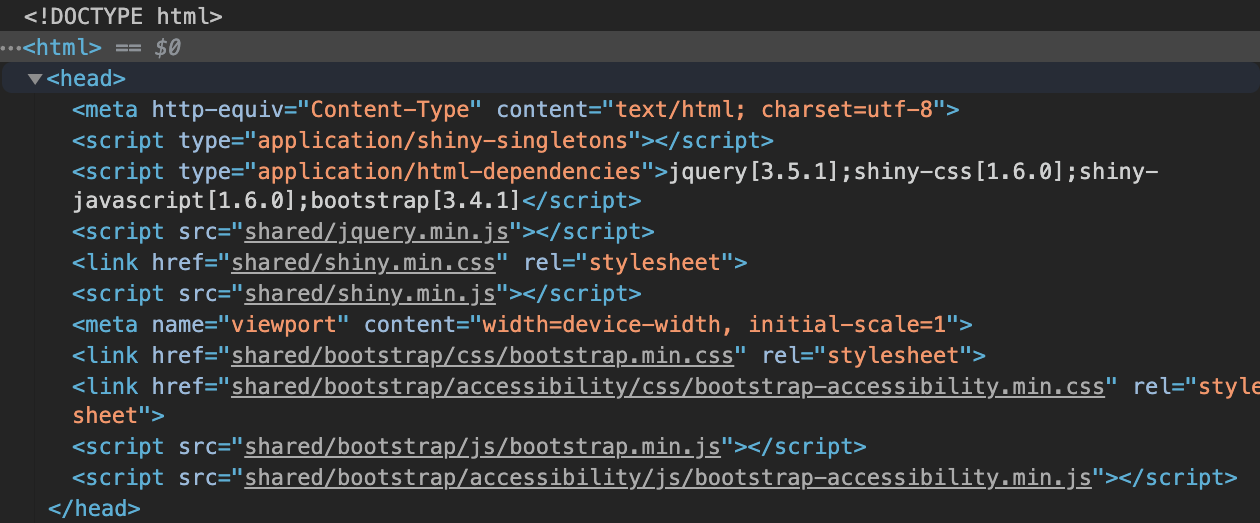
\includegraphics[width=14.92in]{images/survival-kit/shiny-deps} \caption{Shiny dependencies}\label{fig:shiny-deps}
\end{figure}

We see in the head section that Shiny has 4 dependencies:

\begin{itemize}
\tightlist
\item
  json2
\item
  jQuery 3.4.1
\item
  shiny (custom JavaScript and CSS)
\item
  Bootstrap 3.4.1 (JavaScript and CSS) + other files (html5shiv, respond)
\end{itemize}

\href{https://getbootstrap.com}{Bootstrap} is here to provide plug and play design and interactions (tabs, navs). For instance the \texttt{fluidRow} and \texttt{column} functions of Shiny leverage the Bootstrap grid to control how elements are displayed in a page. This is convenient because it avoids to write a crazy amount of CSS/JavaScript and always reinvent the wheel. jQuery drives the DOM manipulations. Shiny has its own JS and CSS files (we will discuss this very soon). Finally, json2 is a library to handle the \href{https://www.json.org/json-en.html}{JSON} data format (JavaScript Object Notation). In the following chapters we will use it a lot, through the jsonlite package that allows to transform JSON objects in R objects and inversely.

In summary, all those libraries are necessary to make Shiny what it is! Customizing Shiny will imply to alter those existing libraries (except the Shiny core JavaScript and json2).

\hypertarget{shiny-hiddens-gems}{%
\section{Shiny hiddens gems}\label{shiny-hiddens-gems}}

As promised earlier, let's talk about the \href{https://github.com/rstudio/shiny/blob/master/srcjs/init_shiny.js}{Shiny JavaScript core}. The goal of this part is to better understand the mechanisms behind Shiny, especially the input system.

\hypertarget{initialization}{%
\subsection{Initialization}\label{initialization}}

Upon initialization, Shiny runs several JavaScript functions. Not surprisingly, there is one called \href{https://github.com/rstudio/shiny/blob/master/srcjs/init_shiny.js}{\texttt{initShiny}} containing a subtantial amount of elements.

We find utils functions like \texttt{bindOutputs}, \texttt{unbindOutputs} to respectively bind/unbind outputs, \texttt{bindInputs} and \texttt{unbindInputs} for inputs. Only \texttt{bindAll} and \texttt{unbindAll} are available to the user (see a usecase \href{https://stackoverflow.com/questions/51633326/dateinput-not-working-on-dt-in-shiny}{here}). To illustrate what they do, let's run the app below.

\begin{Shaded}
\begin{Highlighting}[]
\NormalTok{ui <-}\StringTok{ }\KeywordTok{fluidPage}\NormalTok{(}
  \KeywordTok{sliderInput}\NormalTok{(}\StringTok{"obs"}\NormalTok{, }\StringTok{"Number of observations:"}\NormalTok{,}
    \DataTypeTok{min =} \DecValTok{0}\NormalTok{, }\DataTypeTok{max =} \DecValTok{1000}\NormalTok{, }\DataTypeTok{value =} \DecValTok{500}
\NormalTok{  ),}
  \KeywordTok{plotOutput}\NormalTok{(}\StringTok{"distPlot"}\NormalTok{)}
\NormalTok{)}

\NormalTok{server <-}\StringTok{ }\ControlFlowTok{function}\NormalTok{(input, output, session) \{}
\NormalTok{  output}\OperatorTok{$}\NormalTok{distPlot <-}\StringTok{ }\KeywordTok{renderPlot}\NormalTok{(\{}
    \KeywordTok{hist}\NormalTok{(}\KeywordTok{rnorm}\NormalTok{(input}\OperatorTok{$}\NormalTok{obs))}
\NormalTok{  \})}
\NormalTok{\}}
\KeywordTok{shinyApp}\NormalTok{(ui, server)}
\end{Highlighting}
\end{Shaded}

We then open the HTML inspector and run \texttt{Shiny.unbindAll(document)} (document is the scope, that is where to search). Try to change the slider input. What do you observe? Now let's type \texttt{Shiny.bindAll(document)} and update the slider value. What happens? Magic isn't it? This simply shows that when inputs are not bound, nothing happens so binding inputs is necessary. Let's see below how an input binding works.

\hypertarget{input-bindings}{%
\subsection{Input bindings}\label{input-bindings}}

The input binding is defined by a class living in the \texttt{input\_binding.js} \href{https://github.com/rstudio/shiny/blob/master/srcjs/input_binding.js}{file}.
An input binding allows Shiny to identify each instance of a given input and what you can do with this input. The interesting thing is that if your app contains 10 different sliders, they all share the same input binding! An input binding is an object having the following methods (but not only):

\begin{itemize}
\tightlist
\item
  find(scope): this method specifies how to find the current input element (el) in the DOM. scope refers to the \texttt{document} element. In general, we use jQuery selector to search for a class.
\item
  initialize(el): This is called before the input is bound but not all input need to be initalized. Some API like \href{https://framework7.io}{Framework7} require to almost always have an initialize method (We will see later).
\item
  getValue(el): returns the input value. The way to obtain the value tighly depends on the object and is different for almost all inputs.
\item
  setValue(el, value): This method is used to set the value of the current input.
\item
  receiveMessage(el, data): This method is the JavaScript part of all the \texttt{updateInput} functions. We usually call the setValue method inside.
\item
  subscribe(el, callback): We listen to events telling under which circumstances to change the input value. Some API like Bootstrap explicitly mention those events (like \texttt{hide.bs.tab}, \texttt{shown.bs.tab}, \ldots{}).
\item
  getRatePolicy: when callback is true in the subscribe method, we apply a specific rate policy (\href{https://davidwalsh.name/javascript-debounce-function}{debounce}, throttle). This is useful for instance when we don't want to flood the server with useless update requests. For a slider, we only want to send the value as soon as the range stops moving and not all intermediate values. Those elements are defined \href{https://github.com/rstudio/shiny/blob/master/srcjs/input_rate.js}{here}.
\end{itemize}

At the end of the input binding definition, we register it for Shiny.

\begin{Shaded}
\begin{Highlighting}[]
\KeywordTok{let}\NormalTok{ myBinding }\OperatorTok{=} \KeywordTok{new} \VariableTok{Shiny}\NormalTok{.}\AttributeTok{inputBinding}\NormalTok{()}\OperatorTok{;}
\VariableTok{$}\NormalTok{.}\AttributeTok{extend}\NormalTok{(myBinding}\OperatorTok{,} \OperatorTok{\{}
  \CommentTok{// methods go here}
\OperatorTok{\}}\NormalTok{)}\OperatorTok{;}

\VariableTok{Shiny}\NormalTok{.}\VariableTok{inputBindings}\NormalTok{.}\AttributeTok{register}\NormalTok{(myBinding}\OperatorTok{,} \StringTok{'reference'}\NormalTok{)}\OperatorTok{;}
\end{Highlighting}
\end{Shaded}

Although the Shiny \href{https://shiny.rstudio.com/articles/building-inputs.html}{documentation} mentions a \texttt{Shiny.inputBindings.setPriority} method to handle conflicting bindings, it is better not to use it.

Upon initialization, Shiny calls the \texttt{initializeInputs} function that takes all input bindings and call their initialize method before binding all inputs. Note that once an input has been initialized it has a \texttt{\_shiny\_initialized} tag to avoid initializing it twice. As shown above, the initialize method is not always defined.

TO DO: picture to add visual representation of an input binding

\hypertarget{websocket}{%
\subsection{websocket}\label{websocket}}

How does R (server) and JavaScript (client) communicate? This is a builtin Shiny feature highlighted \href{Fast\%20bidirectional\%20communication\%20between\%20the\%20web\%20browser\%20and\%20R\%20using\%20the\%20httpuv\%20package.}{here}, leveraging the \href{https://github.com/rstudio/httpuv}{httpuv} and \href{https://github.com/rstudio/websocket}{websocket} packages. We will not detail how they work but rather how to inspect the websocket in a web browser. Let's run the following app.

\begin{Shaded}
\begin{Highlighting}[]
\KeywordTok{shinyApp}\NormalTok{(}
  \DataTypeTok{ui =} \KeywordTok{fluidPage}\NormalTok{(}
    \KeywordTok{selectInput}\NormalTok{(}\StringTok{"variable"}\NormalTok{, }\StringTok{"Variable:"}\NormalTok{,}
                \KeywordTok{c}\NormalTok{(}\StringTok{"Cylinders"}\NormalTok{ =}\StringTok{ "cyl"}\NormalTok{,}
                  \StringTok{"Transmission"}\NormalTok{ =}\StringTok{ "am"}\NormalTok{,}
                  \StringTok{"Gears"}\NormalTok{ =}\StringTok{ "gear"}\NormalTok{)),}
    \KeywordTok{tableOutput}\NormalTok{(}\StringTok{"data"}\NormalTok{)}
\NormalTok{  ),}
  \DataTypeTok{server =} \ControlFlowTok{function}\NormalTok{(input, output) \{}
\NormalTok{    output}\OperatorTok{$}\NormalTok{data <-}\StringTok{ }\KeywordTok{renderTable}\NormalTok{(\{}
\NormalTok{      mtcars[, }\KeywordTok{c}\NormalTok{(}\StringTok{"mpg"}\NormalTok{, input}\OperatorTok{$}\NormalTok{variable), drop =}\StringTok{ }\OtherTok{FALSE}\NormalTok{]}
\NormalTok{    \}, }\DataTypeTok{rownames =} \OtherTok{TRUE}\NormalTok{)}
\NormalTok{  \}}
\NormalTok{)}
\end{Highlighting}
\end{Shaded}

After opening the HTML inspector, we select the network tab and search for websocket in the list. We also choose the message tab to inspect what R and JavaScript say to each others. On the JavaScript side, the websocket is created in the shinyapp.js \href{https://github.com/rstudio/shiny/blob/master/srcjs/shinyapp.js}{file}. The first element received from R is the first message in the list shown in Figure \ref{fig:shiny-websocket}. It is a JSON containing the method used as well as passed data. In the meantime, you may change the select input value.

\begin{Shaded}
\begin{Highlighting}[]
\VariableTok{socket}\NormalTok{.}\AttributeTok{send}\NormalTok{(}\VariableTok{JSON}\NormalTok{.}\AttributeTok{stringify}\NormalTok{(}\OperatorTok{\{}
  \DataTypeTok{method}\OperatorTok{:} \StringTok{'init'}\OperatorTok{,}
  \DataTypeTok{data}\OperatorTok{:} \VariableTok{self}\NormalTok{.}\AttributeTok{$initialInput}
\OperatorTok{\}}\NormalTok{))}\OperatorTok{;}
\end{Highlighting}
\end{Shaded}

The second message received from R is after updating the select input.

\begin{Shaded}
\begin{Highlighting}[]
\KeywordTok{this}\NormalTok{.}\AttributeTok{sendInput} \OperatorTok{=} \KeywordTok{function}\NormalTok{(values) }\OperatorTok{\{}
  \KeywordTok{var}\NormalTok{ msg }\OperatorTok{=} \VariableTok{JSON}\NormalTok{.}\AttributeTok{stringify}\NormalTok{(}\OperatorTok{\{}
    \DataTypeTok{method}\OperatorTok{:} \StringTok{'update'}\OperatorTok{,}
    \DataTypeTok{data}\OperatorTok{:}\NormalTok{ values}
  \OperatorTok{\}}\NormalTok{)}\OperatorTok{;}

  \CommentTok{// other things}
\OperatorTok{\};}
\end{Highlighting}
\end{Shaded}

All of this is quite complex but extremely useful to check wether input/output work properly. In case of error, we would see the field \texttt{error} containing some elements. In the last part of this book, we will be designing custom inputs and knowing how to debug them outside R is priceless.

Finally, \texttt{Shiny.shinyapp.\$socket.readyState} returns the state of the socket connection. It should be 1 if your app is running but I've seen some cases where the socket was actually closed (and nothing could happen).

\begin{figure}
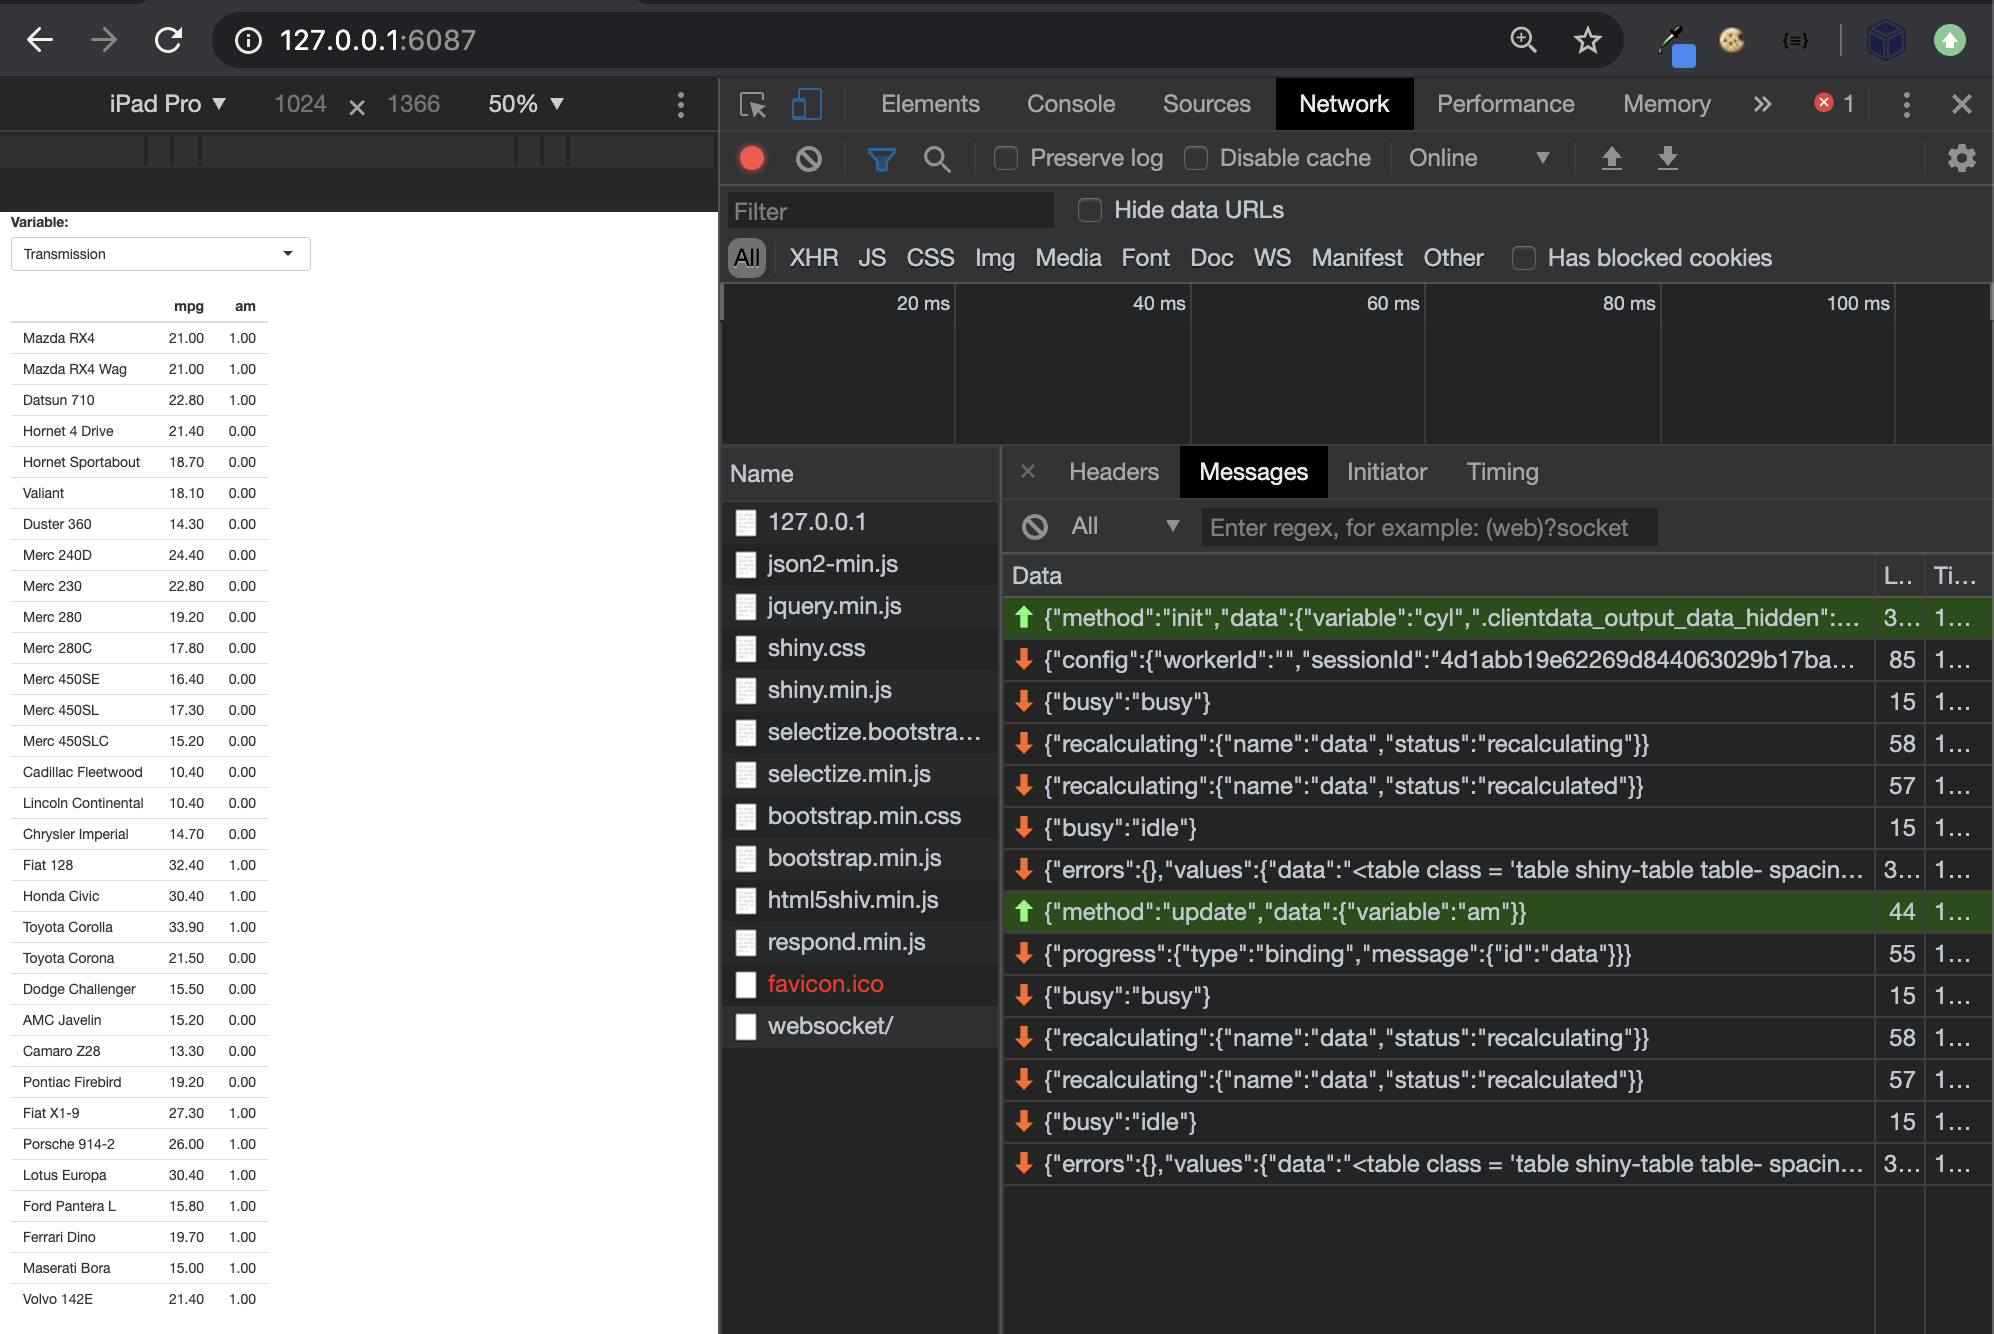
\includegraphics[width=27.69in]{images/survival-kit/shiny-websocket} \caption{Shiny websocket}\label{fig:shiny-websocket}
\end{figure}

\hypertarget{custom-handlers-from-r-to-javascript}{%
\subsection{Custom handlers: from R to JavaScript}\label{custom-handlers-from-r-to-javascript}}

Shiny contains tools to ease the communication between R and JavaScript. This is what happens in the last part. If you remember, we were playing with a \texttt{selectInput} and a \texttt{datatable}. How does R send messages to JavaScript?

Shiny is made of input and output. Yet there is a third parameter you can pass to the server function called session. The \href{https://shiny.rstudio.com/reference/shiny/1.4.0/session.html}{session} object contains informations on the current session like clientData, the namespace ns (if working inside modules), as well as methods (yes methods since session is an R6 class). Among those methods, we are interested by 2 of them:

\begin{itemize}
\tightlist
\item
  \texttt{sendCustomMessage(type,\ message)}: \textgreater{} Custom messages have no meaning to Shiny itself; they are used soley to convey information to custom JavaScript logic in the browser
\item
  \texttt{sendInputMessage()}: \textgreater{} if the input is present and bound on the page at the time the message is received, then the input binding object's receiveMessage(el, message) method will be called
\end{itemize}

While \texttt{sendInputMessage} is the R side of the input features, \texttt{sendCustomMessage} simply allows to communicate between R and JavaScript.
Basically a R function :

\begin{Shaded}
\begin{Highlighting}[]
\NormalTok{sayHelloToJS <-}\StringTok{ }\ControlFlowTok{function}\NormalTok{(text, session) \{}
\NormalTok{  session}\OperatorTok{$}\KeywordTok{sendCustomMessage}\NormalTok{(}\DataTypeTok{type =} \StringTok{'say-hello'}\NormalTok{, }\DataTypeTok{message =}\NormalTok{ text)}
\NormalTok{\}}
\end{Highlighting}
\end{Shaded}

We need a JavaScript receptor, handle by the \texttt{addCustomMessageHandler} method:

\begin{Shaded}
\begin{Highlighting}[]
\VariableTok{Shiny}\NormalTok{.}\AttributeTok{AddCustomMessageHandler}\NormalTok{(}\StringTok{'say-hello'}\OperatorTok{,} \KeywordTok{function}\NormalTok{(message) }\OperatorTok{\{}
  \AttributeTok{alert}\NormalTok{(}\VerbatimStringTok{`R says }\SpecialCharTok{$\{}\NormalTok{message}\SpecialCharTok{\}}\VerbatimStringTok{ to you!`}\NormalTok{)}
\OperatorTok{\}}\NormalTok{)}
\end{Highlighting}
\end{Shaded}

Of course, the type parameter is critical to make the connection between R and JavaScript and 2 different message handlers must have different types to avoid conflicts.

TO DO: picture showing the communication

\hypertarget{utilities-to-quickly-define-new-inputs}{%
\subsection{Utilities to quickly define new inputs}\label{utilities-to-quickly-define-new-inputs}}

If you ever wondered where the \texttt{Shiny.onInputChange} or \texttt{Shiny.setInputValue} comes from (see \href{https://shiny.rstudio.com/articles/communicating-with-js.html}{article}), it is actually defined in the \texttt{initShiny} function.

\begin{Shaded}
\begin{Highlighting}[]
\VariableTok{exports}\NormalTok{.}\AttributeTok{setInputValue} \OperatorTok{=} \VariableTok{exports}\NormalTok{.}\AttributeTok{onInputChange} \OperatorTok{=} \KeywordTok{function}\NormalTok{(name}\OperatorTok{,}\NormalTok{ value}\OperatorTok{,}\NormalTok{ opts) }\OperatorTok{\{}
\NormalTok{  opts }\OperatorTok{=} \AttributeTok{addDefaultInputOpts}\NormalTok{(opts)}\OperatorTok{;}
  \VariableTok{inputs}\NormalTok{.}\AttributeTok{setInput}\NormalTok{(name}\OperatorTok{,}\NormalTok{ value}\OperatorTok{,}\NormalTok{ opts)}\OperatorTok{;}
\OperatorTok{\};}
\end{Highlighting}
\end{Shaded}

Briefly, this function avoids to create an input binding. It is faster to code but there is a price to pay: you lose the possibility to easily update the new input. Indeed, all input functions like \texttt{sliderInput} have their own update function like \texttt{updateSliderInput}, because of the custom input binding system (We will see it very soon)!

\hypertarget{get-access-to-initial-values}{%
\subsection{Get access to initial values}\label{get-access-to-initial-values}}

Something we may notice when exploring the \texttt{initShiny} function is the existence of a shinyapp object, defined as follows:

\begin{Shaded}
\begin{Highlighting}[]
\KeywordTok{var}\NormalTok{ shinyapp }\OperatorTok{=} \VariableTok{exports}\NormalTok{.}\AttributeTok{shinyapp} \OperatorTok{=} \KeywordTok{new} \AttributeTok{ShinyApp}\NormalTok{()}\OperatorTok{;}
\end{Highlighting}
\end{Shaded}

Let's explore what ShinyApp contains. The definition is located in the shinyapps.js \href{https://github.com/rstudio/shiny/blob/master/srcjs/shinyapp.js}{script}.

\begin{Shaded}
\begin{Highlighting}[]
\KeywordTok{var}\NormalTok{ ShinyApp }\OperatorTok{=} \KeywordTok{function}\NormalTok{() }\OperatorTok{\{}
  \KeywordTok{this}\NormalTok{.}\AttributeTok{$socket} \OperatorTok{=} \KeywordTok{null}\OperatorTok{;}

  \CommentTok{// Cached input values}
  \KeywordTok{this}\NormalTok{.}\AttributeTok{$inputValues} \OperatorTok{=} \OperatorTok{\{\};}

  \CommentTok{// Input values at initialization (and reconnect)}
  \KeywordTok{this}\NormalTok{.}\AttributeTok{$initialInput} \OperatorTok{=} \OperatorTok{\{\};}

  \CommentTok{// Output bindings}
  \KeywordTok{this}\NormalTok{.}\AttributeTok{$bindings} \OperatorTok{=} \OperatorTok{\{\};}

  \CommentTok{// Cached values/errors}
  \KeywordTok{this}\NormalTok{.}\AttributeTok{$values} \OperatorTok{=} \OperatorTok{\{\};}
  \KeywordTok{this}\NormalTok{.}\AttributeTok{$errors} \OperatorTok{=} \OperatorTok{\{\};}

  \CommentTok{// Conditional bindings (show/hide element based on expression)}
  \KeywordTok{this}\NormalTok{.}\AttributeTok{$conditionals} \OperatorTok{=} \OperatorTok{\{\};}

  \KeywordTok{this}\NormalTok{.}\AttributeTok{$pendingMessages} \OperatorTok{=}\NormalTok{ []}\OperatorTok{;}
  \KeywordTok{this}\NormalTok{.}\AttributeTok{$activeRequests} \OperatorTok{=} \OperatorTok{\{\};}
  \KeywordTok{this}\NormalTok{.}\AttributeTok{$nextRequestId} \OperatorTok{=} \DecValTok{0}\OperatorTok{;}

  \KeywordTok{this}\NormalTok{.}\AttributeTok{$allowReconnect} \OperatorTok{=} \KeywordTok{false}\OperatorTok{;}
\OperatorTok{\};}
\end{Highlighting}
\end{Shaded}

It creates several properties, some of them are easy to guess like \texttt{inputValues} or \texttt{initialInput}. Let's run the example below and open the HTML inspector. Notice that the \texttt{sliderInput} is set to 500 at \texttt{t0} (initialization).

\begin{Shaded}
\begin{Highlighting}[]
\NormalTok{ui <-}\StringTok{ }\KeywordTok{fluidPage}\NormalTok{(}
  \KeywordTok{sliderInput}\NormalTok{(}\StringTok{"obs"}\NormalTok{, }\StringTok{"Number of observations:"}\NormalTok{,}
    \DataTypeTok{min =} \DecValTok{0}\NormalTok{, }\DataTypeTok{max =} \DecValTok{1000}\NormalTok{, }\DataTypeTok{value =} \DecValTok{500}
\NormalTok{  ),}
  \KeywordTok{plotOutput}\NormalTok{(}\StringTok{"distPlot"}\NormalTok{)}
\NormalTok{)}

\NormalTok{server <-}\StringTok{ }\ControlFlowTok{function}\NormalTok{(input, output, session) \{}
\NormalTok{  output}\OperatorTok{$}\NormalTok{distPlot <-}\StringTok{ }\KeywordTok{renderPlot}\NormalTok{(\{}
    \KeywordTok{hist}\NormalTok{(}\KeywordTok{rnorm}\NormalTok{(input}\OperatorTok{$}\NormalTok{obs))}
\NormalTok{  \})}
\NormalTok{\}}
\KeywordTok{shinyApp}\NormalTok{(ui, server)}
\end{Highlighting}
\end{Shaded}

Figure \ref{fig:shiny-initial-inputs} shows how to access Shiny's initial input value with \texttt{Shiny.shinyapp.\$initialInput.obs}. After changing the slider position, its value is given by \texttt{Shiny.shinyapp.\$inputValues.obs}. \texttt{\$initialInput} and \texttt{\$inputValues} contains way more elements but we are only interested by the slider in this example.

\begin{figure}
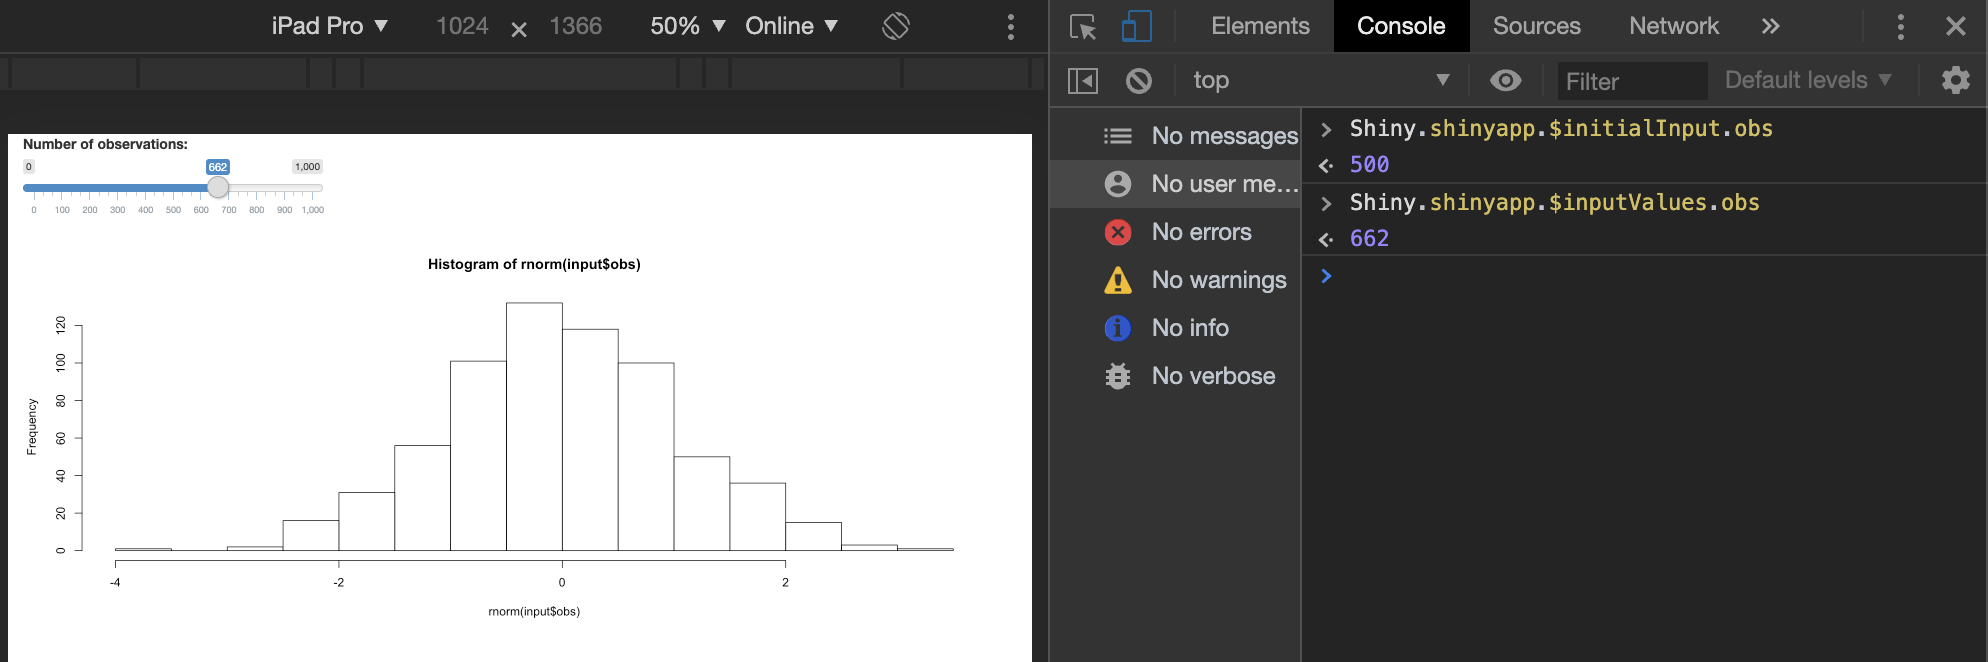
\includegraphics[width=27.61in]{images/survival-kit/shiny-init-input} \caption{Explore initial input values}\label{fig:shiny-initial-inputs}
\end{figure}

I acknowledge, the practical interest might be limited but still good to know for debugging purposes.

\hypertarget{part-htmltools}{%
\part*{htmltools}\label{part-htmltools}}
\addcontentsline{toc}{part}{htmltools}

While building a custom html template, you will need to know more about the wonderful \href{https://github.com/rstudio/htmltools}{htmltools} developed by Winston Chang, member of the shiny core team. It has the same spirit as devtools, that is, making your web developer life easier. What follows does not have the pretention to be an exhaustive guide about this package. Yet, it will provide you yith the main tools to be more efficient.

\hypertarget{htmltools-overview}{%
\chapter{htmltools overview}\label{htmltools-overview}}

\hypertarget{html-tags}{%
\section{HTML Tags}\label{html-tags}}

htmltools contains tools to write HTML tags we saw in Chapter \ref{survival-kit-html}:

\begin{Shaded}
\begin{Highlighting}[]
\KeywordTok{div}\NormalTok{()}
\end{Highlighting}
\end{Shaded}

If you had to gather multiple tags together, prefer \texttt{tagList()} as \texttt{list()}, although the HTML output is the same. The first has the shiny.tag.list class in addition to list. (The \href{http://golemverse.org}{Golem} package allows to test if a R object is a tag list, therefore using list would make the test fail).

\hypertarget{notations}{%
\section{Notations}\label{notations}}

Whether to use \texttt{tags\$div} or \texttt{div} depends if the tag is exported by default.
For instance, you could use \texttt{htmltools::div} but not \texttt{htmltools::nav} since nav does not have a dedicated function (only for p, h1, h2, h3, h4, h5, h6, a, br, div, span, pre, code, img, strong, em, hr).
Rather use \texttt{htmltools::tags\$nav}. Alternatively, there exists a function (in shiny and htmltools)
called \texttt{withTags()}. Wrapping your code in this function enables you to use \texttt{withTags(nav(),\ ...)}
instead of \texttt{tags\$nav()}.

\hypertarget{adding-new-tags}{%
\section{Adding new tags}\label{adding-new-tags}}

The \texttt{tag} function allows to add extra HTML tags not already defined. You may use it as follows:

\begin{Shaded}
\begin{Highlighting}[]
\KeywordTok{tag}\NormalTok{(}\StringTok{"test"}\NormalTok{, }\KeywordTok{list}\NormalTok{(}\DataTypeTok{class =} \StringTok{"test"}\NormalTok{, }\KeywordTok{p}\NormalTok{(}\StringTok{"Custom Tag"}\NormalTok{)))}
\CommentTok{# structure below}
\NormalTok{█─tag }
\NormalTok{├─}\StringTok{"test"} 
\NormalTok{└─█─list }
\NormalTok{├─class =}\StringTok{ "test"} 
\NormalTok{└─█─p }
\NormalTok{└─}\StringTok{"Custom Tag"} 
\end{Highlighting}
\end{Shaded}

\hypertarget{alternative-way-to-write-tags}{%
\section{Alternative way to write tags}\label{alternative-way-to-write-tags}}

htmltools comes with the \texttt{HTML()} function that you can feed with raw HTML:

\begin{Shaded}
\begin{Highlighting}[]
\KeywordTok{HTML}\NormalTok{(}\StringTok{'<div>Blabla</div>'}\NormalTok{)}
\CommentTok{# will render exactly like}
\KeywordTok{div}\NormalTok{(}\StringTok{"Blabla"}\NormalTok{)}

\CommentTok{# but there class is different}
\KeywordTok{class}\NormalTok{(}\KeywordTok{HTML}\NormalTok{(}\StringTok{'<div>Blabla</div>'}\NormalTok{))}
\KeywordTok{class}\NormalTok{(}\KeywordTok{div}\NormalTok{(}\StringTok{"Blabla"}\NormalTok{))}
\end{Highlighting}
\end{Shaded}

You will not be able to use tag related functions, as in the following parts.
Therefore, I strongly recommand using R and not mixing HTML in R. Interestingly, if
you want to convert HTML to R code, there is a Shiny App developed by Alan
Dipert from RStudio, namely \href{https://github.com/alandipert/html2r}{html2R}. There
are some issues, non standard attributes (like \texttt{data-toggle}) are not correctly processed but there are \href{https://github.com/alandipert/html2r/issues/2}{fixes}. This will save you precious time!

\hypertarget{playing-with-tags}{%
\section{Playing with tags}\label{playing-with-tags}}

\hypertarget{tags-structure}{%
\subsection{Tags structure}\label{tags-structure}}

According to the \texttt{tag} function, a tag has:

\begin{itemize}
\tightlist
\item
  a name such as span, div, h1 \ldots{} \texttt{tag\$name}
\item
  some attributes, which you can access with \texttt{tag\$attribs}
\item
  children, which you can access with \texttt{tag\$children}
\item
  a class, namely ``shiny.tag''
\end{itemize}

For instance:

\begin{Shaded}
\begin{Highlighting}[]
\CommentTok{# create the tag}
\NormalTok{myTag <-}\StringTok{ }\KeywordTok{div}\NormalTok{(}
  \DataTypeTok{class =} \StringTok{"divclass"}\NormalTok{, }
  \DataTypeTok{id =} \StringTok{"first"}\NormalTok{,}
  \KeywordTok{h1}\NormalTok{(}\StringTok{"Here comes your baby"}\NormalTok{),}
  \KeywordTok{span}\NormalTok{(}\DataTypeTok{class =} \StringTok{"child"}\NormalTok{, }\DataTypeTok{id =} \StringTok{"baby"}\NormalTok{, }\StringTok{"Crying"}\NormalTok{)}
\NormalTok{)}
\CommentTok{# access its name}
\NormalTok{myTag}\OperatorTok{$}\NormalTok{name}
\CommentTok{# access its attributes (id and class)}
\NormalTok{myTag}\OperatorTok{$}\NormalTok{attribs}
\CommentTok{# access children (returns a list of 2 elements)}
\NormalTok{myTag}\OperatorTok{$}\NormalTok{children}
\CommentTok{# access its class}
\KeywordTok{class}\NormalTok{(myTag)}
\end{Highlighting}
\end{Shaded}

How to modify the class of the second child, namely span?

\begin{Shaded}
\begin{Highlighting}[]
\NormalTok{second_children <-}\StringTok{ }\NormalTok{myTag}\OperatorTok{$}\NormalTok{children[[}\DecValTok{2}\NormalTok{]]}
\NormalTok{second_children}\OperatorTok{$}\NormalTok{attribs}\OperatorTok{$}\NormalTok{class <-}\StringTok{ "adult"}
\NormalTok{myTag}
\CommentTok{# Hummm, this is not working ...}
\end{Highlighting}
\end{Shaded}

Why is this not working? By assigning \texttt{myTag\$children{[}{[}2{]}{]}} to second\_children, \texttt{second\_children\$attribs\$class\ \textless{}-\ "adult"} modifies the class of the copy and not the original object. Thus we do:

\begin{Shaded}
\begin{Highlighting}[]
\NormalTok{myTag}\OperatorTok{$}\NormalTok{children[[}\DecValTok{2}\NormalTok{]]}\OperatorTok{$}\NormalTok{attribs}\OperatorTok{$}\NormalTok{class <-}\StringTok{ "adult"}
\NormalTok{myTag}
\end{Highlighting}
\end{Shaded}

In the following section we explore helper functions, such as \texttt{tagAppendChild} from htmltools.

\hypertarget{useful-functions-for-tags}{%
\subsection{Useful functions for tags}\label{useful-functions-for-tags}}

htmltools and Shiny have powerful functions to easily add attributes to tags, check for existing attributes, get attributes and add other siblings to a list of tags.

\hypertarget{add-attributes}{%
\subsubsection{Add attributes}\label{add-attributes}}

\begin{itemize}
\tightlist
\item
  \texttt{tagAppendAttributes}: this function allow you to add a new attribute to the current tag.
\end{itemize}

For instance, assuming you created a div for which you forgot to add an id attribute:

\begin{Shaded}
\begin{Highlighting}[]
\NormalTok{mydiv <-}\StringTok{ }\KeywordTok{div}\NormalTok{(}\StringTok{"Where is my brain"}\NormalTok{)}
\NormalTok{mydiv <-}\StringTok{ }\KeywordTok{tagAppendAttributes}\NormalTok{(mydiv, }\DataTypeTok{id =} \StringTok{"here_it_is"}\NormalTok{)}
\end{Highlighting}
\end{Shaded}

You can pass as many attributes as you want, including non standard attributes such as \texttt{data-toggle} (see Bootstrap 3 tabs for instance):

\begin{Shaded}
\begin{Highlighting}[]
\NormalTok{mydiv <-}\StringTok{ }\KeywordTok{tagAppendAttributes}\NormalTok{(mydiv, }\StringTok{`}\DataTypeTok{data-toggle}\StringTok{`}\NormalTok{ =}\StringTok{ "tabs"}\NormalTok{)}
\CommentTok{# even though you could proceed as follows}
\NormalTok{mydiv}\OperatorTok{$}\NormalTok{attribs[[}\StringTok{"aria-controls"}\NormalTok{]] <-}\StringTok{ "home"}
\end{Highlighting}
\end{Shaded}

\hypertarget{check-if-tag-has-specific-attribute}{%
\subsubsection{Check if tag has specific attribute}\label{check-if-tag-has-specific-attribute}}

\begin{itemize}
\tightlist
\item
  \texttt{tagHasAttribute}: to check if a tag has a specific attribute
\end{itemize}

\begin{Shaded}
\begin{Highlighting}[]
\CommentTok{# I want to know if div has a class}
\NormalTok{mydiv <-}\StringTok{ }\KeywordTok{div}\NormalTok{(}\DataTypeTok{class =} \StringTok{"myclass"}\NormalTok{)}
\NormalTok{has_class <-}\StringTok{ }\KeywordTok{tagHasAttribute}\NormalTok{(mydiv, }\StringTok{"class"}\NormalTok{)}
\NormalTok{has_class}
\CommentTok{# if you are familiar with %>%}
\NormalTok{has_class <-}\StringTok{ }\NormalTok{mydiv }\OperatorTok\StringTok{ }\KeywordTok{tagHasAttribute}\NormalTok{(}\StringTok{"class"}\NormalTok{)}
\NormalTok{has_class}
\end{Highlighting}
\end{Shaded}

\hypertarget{get-all-attributes}{%
\subsubsection{Get all attributes}\label{get-all-attributes}}

\begin{itemize}
\tightlist
\item
  \texttt{tagGetAttribute}: to get the value of the targeted attributes, if it exists, otherwise NULL.
\end{itemize}

\begin{Shaded}
\begin{Highlighting}[]
\NormalTok{mydiv <-}\StringTok{ }\KeywordTok{div}\NormalTok{(}\DataTypeTok{class =} \StringTok{"test"}\NormalTok{)}
\CommentTok{# returns the class}
\KeywordTok{tagGetAttribute}\NormalTok{(mydiv, }\StringTok{"class"}\NormalTok{)}
\CommentTok{# returns NULL}
\KeywordTok{tagGetAttribute}\NormalTok{(mydiv, }\StringTok{"id"}\NormalTok{)}
\end{Highlighting}
\end{Shaded}

\hypertarget{set-childchildren}{%
\subsubsection{Set child/children}\label{set-childchildren}}

\begin{itemize}
\tightlist
\item
  \texttt{tagSetChildren} allows to create children for a given tag. For instance:
\end{itemize}

\begin{Shaded}
\begin{Highlighting}[]
\NormalTok{mydiv <-}\StringTok{ }\KeywordTok{div}\NormalTok{(}\DataTypeTok{class =} \StringTok{"parent"}\NormalTok{, }\DataTypeTok{id =} \StringTok{"mother"}\NormalTok{, }\StringTok{"Not the mama!!!"}\NormalTok{)}
\CommentTok{# mydiv has 1 child "Not the mama!!!"}
\NormalTok{mydiv }
\NormalTok{children <-}\StringTok{ }\KeywordTok{lapply}\NormalTok{(}\DecValTok{1}\OperatorTok{:}\DecValTok{3}\NormalTok{, span)}
\NormalTok{mydiv <-}\StringTok{ }\KeywordTok{tagSetChildren}\NormalTok{(mydiv, children)}
\CommentTok{# mydiv has 3 children, the first one was removed}
\NormalTok{mydiv }
\end{Highlighting}
\end{Shaded}

Notice that \texttt{tagSetChildren} removes all existing children. Below we see another set of functions to add children while conserving existing ones.

\hypertarget{add-child-or-children}{%
\subsubsection{Add child or children}\label{add-child-or-children}}

\begin{itemize}
\tightlist
\item
  \texttt{tagAppendChild} and \texttt{tagAppendChildren}: add other tags to an existing tag.
  Whereas \texttt{tagAppendChild} only takes one tag, you can pass a list of tags to \texttt{tagAppendChildren}.
\end{itemize}

\begin{Shaded}
\begin{Highlighting}[]
\NormalTok{mydiv <-}\StringTok{ }\KeywordTok{div}\NormalTok{(}\DataTypeTok{class =} \StringTok{"parent"}\NormalTok{, }\DataTypeTok{id =} \StringTok{"mother"}\NormalTok{, }\StringTok{"Not the mama!!!"}\NormalTok{)}
\NormalTok{otherTag <-}\StringTok{ }\KeywordTok{span}\NormalTok{(}\StringTok{"I am your child"}\NormalTok{)}
\NormalTok{mydiv <-}\StringTok{ }\KeywordTok{tagAppendChild}\NormalTok{(mydiv, otherTag)}
\end{Highlighting}
\end{Shaded}

You might wonder why there is no \texttt{tagRemoveChild} or \texttt{tagRemoveAttributes}.
Let's look at the \texttt{tagAppendChild}

\begin{Shaded}
\begin{Highlighting}[]
\NormalTok{tagAppendChild <-}\StringTok{ }\ControlFlowTok{function}\NormalTok{ (tag, child) \{}
\NormalTok{  tag}\OperatorTok{$}\NormalTok{children[[}\KeywordTok{length}\NormalTok{(tag}\OperatorTok{$}\NormalTok{children) }\OperatorTok{+}\StringTok{ }\DecValTok{1}\NormalTok{]] <-}\StringTok{ }\NormalTok{child}
\NormalTok{  tag}
\NormalTok{\}}
\end{Highlighting}
\end{Shaded}

Below we write the \texttt{tagRemoveChild}, where tag is the target and n is the position to remove in the list of children:

\begin{Shaded}
\begin{Highlighting}[]
\NormalTok{mydiv <-}\StringTok{ }\KeywordTok{div}\NormalTok{(}\DataTypeTok{class =} \StringTok{"parent"}\NormalTok{, }\DataTypeTok{id =} \StringTok{"mother"}\NormalTok{, }\StringTok{"Not the mama!!!"}\NormalTok{, }\KeywordTok{span}\NormalTok{(}\StringTok{"Hey!"}\NormalTok{))}

\CommentTok{# we create the tagRemoveChild function}
\NormalTok{tagRemoveChild <-}\StringTok{ }\ControlFlowTok{function}\NormalTok{(tag, n) \{}
  \CommentTok{# check if the list is empty}
  \ControlFlowTok{if}\NormalTok{ (}\KeywordTok{length}\NormalTok{(tag}\OperatorTok{$}\NormalTok{children) }\OperatorTok{==}\StringTok{ }\DecValTok{0}\NormalTok{) \{}
    \KeywordTok{stop}\NormalTok{(}\KeywordTok{paste}\NormalTok{(tag}\OperatorTok{$}\NormalTok{name, }\StringTok{"does not have any children!"}\NormalTok{))}
\NormalTok{  \}}
\NormalTok{  tag}\OperatorTok{$}\NormalTok{children[n] <-}\StringTok{ }\OtherTok{NULL}
\NormalTok{  tag}
\NormalTok{\}}
\NormalTok{mydiv <-}\StringTok{ }\KeywordTok{tagRemoveChild}\NormalTok{(mydiv, }\DecValTok{1}\NormalTok{)}
\NormalTok{mydiv}
\end{Highlighting}
\end{Shaded}

When defining the \texttt{tagRemoveChild}, we choose \texttt{{[}} instead of \texttt{{[}{[}} to allow to select multiple list elements:

\begin{Shaded}
\begin{Highlighting}[]
\NormalTok{mydiv <-}\StringTok{ }\KeywordTok{div}\NormalTok{(}\DataTypeTok{class =} \StringTok{"parent"}\NormalTok{, }\DataTypeTok{id =} \StringTok{"mother"}\NormalTok{, }\StringTok{"Not the mama!!!"}\NormalTok{, }\StringTok{"Hey!"}\NormalTok{)}
\CommentTok{# fails}
\StringTok{`}\DataTypeTok{[[}\StringTok{`}\NormalTok{(mydiv}\OperatorTok{$}\NormalTok{children, }\KeywordTok{c}\NormalTok{(}\DecValTok{1}\NormalTok{, }\DecValTok{2}\NormalTok{))}
\CommentTok{# works}
\StringTok{`}\DataTypeTok{[}\StringTok{`}\NormalTok{(mydiv}\OperatorTok{$}\NormalTok{children, }\KeywordTok{c}\NormalTok{(}\DecValTok{1}\NormalTok{, }\DecValTok{2}\NormalTok{))}
\end{Highlighting}
\end{Shaded}

Alternatively, we could also create a \texttt{tagRemoveChildren} function. Also notice that the function raises an error if the provided tag does not have children.

\hypertarget{other-interesting-functions}{%
\subsection{Other interesting functions}\label{other-interesting-functions}}

The \href{https://github.com/ThinkR-open/golem/blob/dev/inst/utils/golem_utils_ui.R}{Golem} package written by \href{https://thinkr.fr}{thinkr} contains neat functions to edit your tags.

Particularly, the \texttt{tagRemoveAttributes}:

\begin{Shaded}
\begin{Highlighting}[]
\NormalTok{tagRemoveAttributes <-}\StringTok{ }\ControlFlowTok{function}\NormalTok{(tag, ...) \{}
\NormalTok{  attrs <-}\StringTok{ }\KeywordTok{as.character}\NormalTok{(}\KeywordTok{list}\NormalTok{(...))}
  \ControlFlowTok{for}\NormalTok{ (i }\ControlFlowTok{in} \KeywordTok{seq_along}\NormalTok{(attrs)) \{}
\NormalTok{    tag}\OperatorTok{$}\NormalTok{attribs[[ attrs[i] ]] <-}\StringTok{ }\OtherTok{NULL}
\NormalTok{  \}}
\NormalTok{  tag}
\NormalTok{\}}
\end{Highlighting}
\end{Shaded}

\begin{Shaded}
\begin{Highlighting}[]
\NormalTok{mydiv <-}\StringTok{ }\KeywordTok{div}\NormalTok{(}\DataTypeTok{class =} \StringTok{"test"}\NormalTok{, }\DataTypeTok{id =} \StringTok{"coucou"}\NormalTok{, }\StringTok{"Hello"}\NormalTok{)}
\KeywordTok{tagRemoveAttributes}\NormalTok{(mydiv, }\StringTok{"class"}\NormalTok{, }\StringTok{"id"}\NormalTok{)}
\end{Highlighting}
\end{Shaded}

\hypertarget{conditionally-set-attributes}{%
\subsection{Conditionally set attributes}\label{conditionally-set-attributes}}

Sometimes, you only want to set attributes under specific conditions.

\begin{Shaded}
\begin{Highlighting}[]
\NormalTok{my_button <-}\StringTok{ }\ControlFlowTok{function}\NormalTok{(}\DataTypeTok{color =} \OtherTok{NULL}\NormalTok{) \{}
\NormalTok{  tags}\OperatorTok{$}\KeywordTok{button}\NormalTok{( }
    \DataTypeTok{style =} \KeywordTok{paste}\NormalTok{(}\StringTok{"color:"}\NormalTok{, color),}
    \KeywordTok{p}\NormalTok{(}\StringTok{"Hello"}\NormalTok{)}
\NormalTok{  )}
\NormalTok{\}}

\KeywordTok{my_button}\NormalTok{()}
\end{Highlighting}
\end{Shaded}

This example will not fail but having \texttt{style="color:\ "} is not clean. We may use conditions:

\begin{Shaded}
\begin{Highlighting}[]
\NormalTok{my_button <-}\StringTok{ }\ControlFlowTok{function}\NormalTok{(}\DataTypeTok{color =} \OtherTok{NULL}\NormalTok{) \{}
\NormalTok{  tags}\OperatorTok{$}\KeywordTok{button}\NormalTok{( }
    \DataTypeTok{style =} \ControlFlowTok{if}\NormalTok{ (}\OperatorTok{!}\KeywordTok{is.null}\NormalTok{(color)) }\KeywordTok{paste}\NormalTok{(}\StringTok{"color:"}\NormalTok{, color),}
    \KeywordTok{p}\NormalTok{(}\StringTok{"Hello"}\NormalTok{)}
\NormalTok{  )}
\NormalTok{\}}

\KeywordTok{my_button}\NormalTok{(}\StringTok{"blue"}\NormalTok{)}
\KeywordTok{my_button}\NormalTok{()}
\end{Highlighting}
\end{Shaded}

In this example, style won't be available if color is not specified.

\hypertarget{using}{%
\subsection{Using \%\textgreater{}\%}\label{using}}

While doing a lot of manipulation for a tag, if you don't need to create intermediate
objects, this is a good idea to use \texttt{\%\textgreater{}\%} from magrittr:

\begin{Shaded}
\begin{Highlighting}[]
\KeywordTok{div}\NormalTok{(}\DataTypeTok{class =} \StringTok{"cl"}\NormalTok{, }\KeywordTok{h1}\NormalTok{(}\StringTok{"Hello"}\NormalTok{)) }\OperatorTok\StringTok{ }
\StringTok{  }\KeywordTok{tagAppendAttributes}\NormalTok{(}\DataTypeTok{id =} \StringTok{"myid"}\NormalTok{) }\OperatorTok
\StringTok{  }\KeywordTok{tagAppendChild}\NormalTok{(}\KeywordTok{p}\NormalTok{(}\StringTok{"some extra text here!"}\NormalTok{))}
\end{Highlighting}
\end{Shaded}

\hypertarget{programmatically-create-children-elements}{%
\subsection{Programmatically create children elements}\label{programmatically-create-children-elements}}

Assume you want to create a tag with 3 children inside:

\begin{Shaded}
\begin{Highlighting}[]
\KeywordTok{div}\NormalTok{(}
  \KeywordTok{span}\NormalTok{(}\DecValTok{1}\NormalTok{),}
  \KeywordTok{span}\NormalTok{(}\DecValTok{2}\NormalTok{),}
  \KeywordTok{span}\NormalTok{(}\DecValTok{3}\NormalTok{),}
  \KeywordTok{span}\NormalTok{(}\DecValTok{4}\NormalTok{),}
  \KeywordTok{span}\NormalTok{(}\DecValTok{5}\NormalTok{)}
\NormalTok{)}
\end{Highlighting}
\end{Shaded}

The structure is correct but imagine if you had to create 1000 \texttt{span} or fancier tag. The previous approach is not consistent with DRY programming. \texttt{lapply} function will be useful here (or the purrr \texttt{map} family):

\begin{Shaded}
\begin{Highlighting}[]
\CommentTok{# base R}
\KeywordTok{div}\NormalTok{(}\KeywordTok{lapply}\NormalTok{(}\DecValTok{1}\OperatorTok{:}\DecValTok{5}\NormalTok{, }\ControlFlowTok{function}\NormalTok{(i) }\KeywordTok{span}\NormalTok{(i)))}
\CommentTok{# purrr + %>%}
\KeywordTok{map}\NormalTok{(}\DecValTok{1}\OperatorTok{:}\DecValTok{5}\NormalTok{, }\ControlFlowTok{function}\NormalTok{(i) }\KeywordTok{span}\NormalTok{(i)) }\OperatorTok\StringTok{ }\KeywordTok{div}\NormalTok{()}
\end{Highlighting}
\end{Shaded}

\hypertarget{htmltools-dependencies}{%
\chapter{Dependency utilities}\label{htmltools-dependencies}}

When creating a new template, you sometimes need to import custom HTML dependencies
that do not come along with shiny. No problem, htmltools is here for you (shiny also
contains these functions).

\hypertarget{the-dirty-approach}{%
\section{The dirty approach}\label{the-dirty-approach}}

Let's consider the following example. I want to include a bootstrap 4 card in a shiny app.
This example is taken from an interesting question \href{https://community.rstudio.com/t/create-a-div-using-htmltools-withtags/22439/2}{here}.
The naive approach would be to include the HTML code directly in the app code

\begin{Shaded}
\begin{Highlighting}[]
\CommentTok{# we create the card function before}
\NormalTok{my_card <-}\StringTok{ }\ControlFlowTok{function}\NormalTok{(...) \{}
  \KeywordTok{withTags}\NormalTok{(}
    \KeywordTok{div}\NormalTok{(}
      \DataTypeTok{class =} \StringTok{"card border-success mb-3"}\NormalTok{,}
      \KeywordTok{div}\NormalTok{(}\DataTypeTok{class =} \StringTok{"card-header bg-transparent border-success"}\NormalTok{),}
      \KeywordTok{div}\NormalTok{(}
        \DataTypeTok{class =} \StringTok{"card-body text-success"}\NormalTok{,}
        \KeywordTok{h3}\NormalTok{(}\DataTypeTok{class =} \StringTok{"card-title"}\NormalTok{, }\StringTok{"title"}\NormalTok{),}
        \KeywordTok{p}\NormalTok{(}\DataTypeTok{class =} \StringTok{"card-text"}\NormalTok{, ...)}
\NormalTok{      ),}
      \KeywordTok{div}\NormalTok{(}\DataTypeTok{class =} \StringTok{"card-footer bg-transparent border-success"}\NormalTok{, }\StringTok{"footer"}\NormalTok{)}
\NormalTok{    )}
\NormalTok{  )}
\NormalTok{\}}

\CommentTok{# we build our app}
\KeywordTok{shinyApp}\NormalTok{(}
  \DataTypeTok{ui =} \KeywordTok{fluidPage}\NormalTok{(}
    \KeywordTok{fluidRow}\NormalTok{(}
      \KeywordTok{column}\NormalTok{(}
        \DataTypeTok{width =} \DecValTok{6}\NormalTok{,}
        \DataTypeTok{align =} \StringTok{"center"}\NormalTok{,}
        \KeywordTok{br}\NormalTok{(),}
        \KeywordTok{my_card}\NormalTok{(}\StringTok{"blablabla. PouetPouet Pouet."}\NormalTok{)}
\NormalTok{      )}
\NormalTok{    )}
\NormalTok{  ),}
  \DataTypeTok{server =} \ControlFlowTok{function}\NormalTok{(input, output) \{\}}
\NormalTok{)}
\end{Highlighting}
\end{Shaded}

and desesperately see that nothing is displayed. If you remember, this was expected since
shiny does not contain bootstrap 4 dependencies and this card is unfortunately a
bootstrap 4 object. Don't panic! We just need to tell shiny to load the css we need to display
this card (if required, we could include the javascript as well). We could use either
\texttt{includeCSS()}, \texttt{tags\$head(tags\$link(rel\ =\ "stylesheet",\ type\ =\ "text/css",\ href\ =\ "custom.css"))}. See
more \href{https://shiny.rstudio.com/articles/css.html}{here}.

\begin{Shaded}
\begin{Highlighting}[]
\KeywordTok{shinyApp}\NormalTok{(}
  \DataTypeTok{ui =} \KeywordTok{fluidPage}\NormalTok{(}
    \CommentTok{# load the css code}
    \KeywordTok{includeCSS}\NormalTok{(}\DataTypeTok{path =} \StringTok{"https://maxcdn.bootstrapcdn.com/bootstrap/4.0.0/css/bootstrap.min.css"}\NormalTok{),}
    \KeywordTok{fluidRow}\NormalTok{(}
      \KeywordTok{column}\NormalTok{(}
        \DataTypeTok{width =} \DecValTok{6}\NormalTok{,}
        \DataTypeTok{align =} \StringTok{"center"}\NormalTok{,}
        \KeywordTok{br}\NormalTok{(),}
        \KeywordTok{my_card}\NormalTok{(}\StringTok{"blablabla. PouetPouet Pouet."}\NormalTok{)}
\NormalTok{      )}
\NormalTok{    )}
\NormalTok{  ),}
  \DataTypeTok{server =} \ControlFlowTok{function}\NormalTok{(input, output) \{\}}
\NormalTok{)}
\end{Highlighting}
\end{Shaded}

The card is ugly (which is another problem we will fix later) but at least displayed.

When I say this approach is dirty, it is because it will not be easily re-usable by others.
Instead, we prefer a packaging approach, like in the next section.

\hypertarget{the-clean-approach}{%
\section{The clean approach}\label{the-clean-approach}}

We will use the \texttt{htmlDependency} and \texttt{attachDependencies} functions from htmltools.
The htmlDependency takes several arguments:

\begin{itemize}
\tightlist
\item
  the name of your dependency
\item
  the version (useful to remember on which version it is built upon)
\item
  a path to the dependency (can be a CDN or a local folder)
\item
  script and stylesheet to respectively pass css and scripts
\end{itemize}

\begin{Shaded}
\begin{Highlighting}[]
\CommentTok{# handle dependency}
\NormalTok{card_css <-}\StringTok{ "bootstrap.min.css"}
\NormalTok{bs4_card_dep <-}\StringTok{ }\ControlFlowTok{function}\NormalTok{() \{}
  \KeywordTok{htmlDependency}\NormalTok{(}
    \DataTypeTok{name =} \StringTok{"bs4_card"}\NormalTok{,}
    \DataTypeTok{version =} \StringTok{"1.0"}\NormalTok{,}
    \DataTypeTok{src =} \KeywordTok{c}\NormalTok{(}\DataTypeTok{href =} \StringTok{"https://maxcdn.bootstrapcdn.com/bootstrap/4.0.0/css/"}\NormalTok{),}
    \DataTypeTok{stylesheet =}\NormalTok{ card_css}
\NormalTok{  )}
\NormalTok{\}}
\end{Highlighting}
\end{Shaded}

We create the card tag and give it the bootstrap 4 dependency through the \texttt{attachDependencies()} function. In recent version of htmltools, we may simply use
\texttt{tagList(tag,\ deps)} instead.

\begin{Shaded}
\begin{Highlighting}[]
\CommentTok{# create the card}
\NormalTok{my_card <-}\StringTok{ }\ControlFlowTok{function}\NormalTok{(...) \{}
\NormalTok{  cardTag <-}\StringTok{ }\KeywordTok{withTags}\NormalTok{(}
    \KeywordTok{div}\NormalTok{(}
      \DataTypeTok{class =} \StringTok{"card border-success mb-3"}\NormalTok{,}
      \KeywordTok{div}\NormalTok{(}\DataTypeTok{class =} \StringTok{"card-header bg-transparent border-success"}\NormalTok{),}
      \KeywordTok{div}\NormalTok{(}
        \DataTypeTok{class =} \StringTok{"card-body text-success"}\NormalTok{,}
        \KeywordTok{h3}\NormalTok{(}\DataTypeTok{class =} \StringTok{"card-title"}\NormalTok{, }\StringTok{"title"}\NormalTok{),}
        \KeywordTok{p}\NormalTok{(}\DataTypeTok{class =} \StringTok{"card-text"}\NormalTok{, ...)}
\NormalTok{      ),}
      \KeywordTok{div}\NormalTok{(}\DataTypeTok{class =} \StringTok{"card-footer bg-transparent border-success"}\NormalTok{, }\StringTok{"footer"}\NormalTok{)}
\NormalTok{    )}
\NormalTok{  )}
  
  \CommentTok{# attach dependencies (old way)}
  \CommentTok{# htmltools::attachDependencies(cardTag, bs4_card_dep())}
  
  \CommentTok{# simpler way}
  \KeywordTok{tagList}\NormalTok{(cardTag, }\KeywordTok{bs4_card_dep}\NormalTok{())}
  
\NormalTok{\}}
\end{Highlighting}
\end{Shaded}

We finally run our app:

\begin{Shaded}
\begin{Highlighting}[]
\CommentTok{# run shiny app }
\NormalTok{ui <-}\StringTok{ }\KeywordTok{fluidPage}\NormalTok{(}
  \DataTypeTok{title =} \StringTok{"Hello Shiny!"}\NormalTok{,}
  \KeywordTok{fluidRow}\NormalTok{(}
    \KeywordTok{column}\NormalTok{(}
      \DataTypeTok{width =} \DecValTok{6}\NormalTok{,}
      \DataTypeTok{align =} \StringTok{"center"}\NormalTok{,}
      \KeywordTok{br}\NormalTok{(),}
      \KeywordTok{my_card}\NormalTok{(}\StringTok{"blablabla. PouetPouet Pouet."}\NormalTok{)}
\NormalTok{    )}
\NormalTok{  )}
\NormalTok{)}

\KeywordTok{shinyApp}\NormalTok{(ui, }\DataTypeTok{server =} \ControlFlowTok{function}\NormalTok{(input, output) \{ \})}
\end{Highlighting}
\end{Shaded}

With this approach, you could develop a package of custom dependencies that people
could use when they need to add custom elements in shiny.

\hypertarget{another-example-importing-html-dependencies-from-other-packages}{%
\section{Another example: Importing HTML dependencies from other packages}\label{another-example-importing-html-dependencies-from-other-packages}}

You may know shinydashboard, a package to design dashboards with shiny. In the following, we would like to integrate the box component in a classic Shiny App (without the dashboard layout). However, if you try to include the Shinydashboard box tag, you will notice that nothing is displayed since Shiny does not have shinydashboard dependencies. Fortunately htmltools contains a function, namely \texttt{findDependencies} that looks for all dependencies attached to a tag. How about extracting shinydashboard dependencies? Before going futher, let's define the basic skeleton of a shinydashboard:

\begin{Shaded}
\begin{Highlighting}[]
\KeywordTok{shinyApp}\NormalTok{(}
  \DataTypeTok{ui =} \KeywordTok{dashboardPage}\NormalTok{(}
    \KeywordTok{dashboardHeader}\NormalTok{(),}
    \KeywordTok{dashboardSidebar}\NormalTok{(),}
    \KeywordTok{dashboardBody}\NormalTok{(),}
    \DataTypeTok{title =} \StringTok{"Dashboard example"}
\NormalTok{  ),}
  \DataTypeTok{server =} \ControlFlowTok{function}\NormalTok{(input, output) \{ \}}
\NormalTok{)}
\end{Highlighting}
\end{Shaded}

We don't need to understand shinydashboard details. However, if you are interested to dig in, \href{https://rstudio.github.io/shinydashboard/}{help yourself}. What is important here is the main
wrapper function \texttt{dashboardPage}. (You should already be familiar with \texttt{fluidPage}, another wrapper function). We apply \texttt{findDependencies} on \texttt{dashboardPage}.

\begin{Shaded}
\begin{Highlighting}[]
\NormalTok{deps <-}\StringTok{ }\KeywordTok{findDependencies}\NormalTok{(}
  \KeywordTok{dashboardPage}\NormalTok{(}
    \DataTypeTok{header =} \KeywordTok{dashboardHeader}\NormalTok{(), }
    \DataTypeTok{sidebar =} \KeywordTok{dashboardSidebar}\NormalTok{(), }
    \DataTypeTok{body =} \KeywordTok{dashboardBody}\NormalTok{()}
\NormalTok{  )}
\NormalTok{)}
\NormalTok{deps}
\end{Highlighting}
\end{Shaded}

deps is a list containg 4 dependencies:

\begin{itemize}
\tightlist
\item
  \href{https://fontawesome.com}{Font Awesome} handles icons
\item
  \href{https://getbootstrap.com/docs/3.3/}{Bootstrap} is the main HTML/CSS/JS template. Importantly,
  please note the version 3.3.7, whereas the current is 4.3.1
\item
  \href{https://adminlte.io}{AdminLTE} is the dependency containg HTML/CSS/JS related to the admin template.
  It is closely linked to Bootstrap 3.
\item
  shinydashboard, the CSS and javascript necessary for shinydashboard to work properly. In practice,
  integrating custom HTML templates to shiny does not usually work out of the box for many reasons (Explain why!) and some modifications are necessary.
\end{itemize}

\begin{verbatim}
[[1]]
List of 10
$ name      : chr "font-awesome"
$ version   : chr "5.3.1"
$ src       :List of 1
..$ file: chr "www/shared/fontawesome"
$ meta      : NULL
$ script    : NULL
$ stylesheet: chr [1:2] "css/all.min.css" "css/v4-shims.min.css"
$ head      : NULL
$ attachment: NULL
$ package   : chr "shiny"
$ all_files : logi TRUE
- attr(*, "class")= chr "html_dependency"
[[2]]
List of 10
$ name      : chr "bootstrap"
$ version   : chr "3.3.7"
$ src       :List of 2
..$ href: chr "shared/bootstrap"
..$ file: chr "/Library/Frameworks/R.framework/Versions/3.5/Resources/library/shiny/www/shared/bootstrap"
$ meta      :List of 1
..$ viewport: chr "width=device-width, initial-scale=1"
$ script    : chr [1:3] "js/bootstrap.min.js" "shim/html5shiv.min.js" "shim/respond.min.js"
$ stylesheet: chr "css/bootstrap.min.css"
$ head      : NULL
$ attachment: NULL
$ package   : NULL
$ all_files : logi TRUE
- attr(*, "class")= chr "html_dependency"
[[3]]
List of 10
$ name      : chr "AdminLTE"
$ version   : chr "2.0.6"
$ src       :List of 1
..$ file: chr "/Library/Frameworks/R.framework/Versions/3.5/Resources/library/shinydashboard/AdminLTE"
$ meta      : NULL
$ script    : chr "app.min.js"
$ stylesheet: chr [1:2] "AdminLTE.min.css" "_all-skins.min.css"
$ head      : NULL
$ attachment: NULL
$ package   : NULL
$ all_files : logi TRUE
- attr(*, "class")= chr "html_dependency"
[[4]]
List of 10
$ name      : chr "shinydashboard"
$ version   : chr "0.7.1"
$ src       :List of 1
..$ file: chr "/Library/Frameworks/R.framework/Versions/3.5/Resources/library/shinydashboard"
$ meta      : NULL
$ script    : chr "shinydashboard.min.js"
$ stylesheet: chr "shinydashboard.css"
$ head      : NULL
$ attachment: NULL
$ package   : NULL
$ all_files : logi TRUE
- attr(*, "class")= chr "html_dependency"
\end{verbatim}

Below, we attach the dependencies to the \texttt{box} with \texttt{tagList}, as shown above. Notice that our custom \texttt{box} does not contain all parameters from shinydashboard but this is not what matters in this example.

\begin{Shaded}
\begin{Highlighting}[]
\NormalTok{my_box <-}\StringTok{ }\ControlFlowTok{function}\NormalTok{(title, status) \{}
  \KeywordTok{tagList}\NormalTok{(}\KeywordTok{box}\NormalTok{(}\DataTypeTok{title =}\NormalTok{ title, }\DataTypeTok{status =}\NormalTok{ status), deps)}
\NormalTok{\}}
\NormalTok{ui <-}\StringTok{ }\KeywordTok{fluidPage}\NormalTok{(}
  \KeywordTok{titlePanel}\NormalTok{(}\StringTok{"Shiny with a box"}\NormalTok{),}
  \KeywordTok{my_box}\NormalTok{(}\DataTypeTok{title =} \StringTok{"My box"}\NormalTok{, }\DataTypeTok{status =} \StringTok{"danger"}\NormalTok{),}
\NormalTok{)}
\NormalTok{server <-}\StringTok{ }\ControlFlowTok{function}\NormalTok{(input, output) \{\}}
\KeywordTok{shinyApp}\NormalTok{(ui, server)}
\end{Highlighting}
\end{Shaded}

Now, you may imagine the possibilities are almost unlimited! Interestingly, this
is the approach we use in \href{https://github.com/dreamRs/shinyWidgets/blob/master/R/useBs4Dash.R}{shinyWidgets} for
the \texttt{useBs4Dash} function and other related tools.

\hypertarget{suppress-dependencies}{%
\section{Suppress dependencies}\label{suppress-dependencies}}

In rare cases, you may need to remove an existing dependency (conflict). The \texttt{suppressDependencies} function allows to perform that task. For instance, \href{https://github.com/Appsilon/shiny.semantic}{shiny.semantic} built on top of
semantic ui is not compatible with Bootstrap. Below, we remove the AdminLTE dependency
from a shinydashboard page and nothing is displayed (as expected):

\begin{Shaded}
\begin{Highlighting}[]
\KeywordTok{shinyApp}\NormalTok{(}
  \DataTypeTok{ui =} \KeywordTok{dashboardPage}\NormalTok{(}
    \KeywordTok{dashboardHeader}\NormalTok{(),}
    \KeywordTok{dashboardSidebar}\NormalTok{(),}
    \KeywordTok{dashboardBody}\NormalTok{(}\KeywordTok{suppressDependencies}\NormalTok{(}\StringTok{"AdminLTE"}\NormalTok{)),}
    \DataTypeTok{title =} \StringTok{"Dashboard example"}
\NormalTok{  ),}
  \DataTypeTok{server =} \ControlFlowTok{function}\NormalTok{(input, output) \{ \}}
\NormalTok{)}
\end{Highlighting}
\end{Shaded}

\hypertarget{htmltools-other-tools}{%
\chapter{Other tools}\label{htmltools-other-tools}}

\hypertarget{css}{%
\section{CSS}\label{css}}

\begin{itemize}
\tightlist
\item
  See \href{https://github.com/nteetor/cascadess}{cascadess} to customize the style of tags
\end{itemize}

\begin{Shaded}
\begin{Highlighting}[]
\NormalTok{ui <-}\StringTok{ }\KeywordTok{list}\NormalTok{(}
  \KeywordTok{cascadess}\NormalTok{(),}
  \KeywordTok{h4}\NormalTok{(}
\NormalTok{    .style }\OperatorTok
\StringTok{      }\KeywordTok{font}\NormalTok{(}\DataTypeTok{case =} \StringTok{"upper"}\NormalTok{) }\OperatorTok
\StringTok{      }\KeywordTok{border}\NormalTok{(}\DataTypeTok{bottom =} \StringTok{"red"}\NormalTok{),}
    \StringTok{"Etiam vel tortor sodales tellus ultricies commodo."}
\NormalTok{  )}
\NormalTok{)}
\end{Highlighting}
\end{Shaded}

\hypertarget{part-practice}{%
\part*{Practice}\label{part-practice}}
\addcontentsline{toc}{part}{Practice}

In this chapter, you will learn how to build your own html templates taken from the web and package them, so that they can be re-used at any time by anybody.

\hypertarget{custom-templates-selection}{%
\chapter{Template selection}\label{custom-templates-selection}}

There exists tons of HTML templates over the web. However, only a few part will be suitable for shiny, mainly because of what follows:

\begin{itemize}
\tightlist
\item
  shiny is built on top of \href{https://getbootstrap.com/docs/3.3/}{Bootstrap 3} (HTML, CSS and Javascript framework), meaning that going for another framework might not be straightforward. However, shinymaterial and shiny.semantic are good examples showing this can be possible.
\item
  shiny relies on \href{https://jquery.com}{jQuery} (currently v 3.4.1 for shiny). Consequently, all templates based upon React, Vue and other Javascript framework will not be natively supported. Again, there exist some \href{https://github.com/alandipert/react-widget-demo/blob/master/app.R}{examples} for React with shiny and more generally,
  the \href{https://react-r.github.io/reactR/}{reactR} package developed by Kent Russell and Alan Dipert from RStudio.
\end{itemize}

See \href{https://github.com/rstudio/shiny/tree/master/inst/www/shared}{the github repository} for more details about all dependencies related to the shiny package.

\begin{quote}
Notes: As shiny depends on Bootstrap 3.4.1, we recommand the user who would like to experiment Bootstrap 4 features to be particularly careful about potential incompatibilies. See a working example here with \href{https://github.com/RinteRface/bs4Dash}{bs4Dash}.
\end{quote}

A good source of \textbf{open source} HTML templates is \href{https://colorlib.com}{Colorlib} and \href{https://www.creative-tim.com/bootstrap-themes/free}{Creative Tim}.

In the next chapter, we will focus on the \href{https://preview-dev.tabler.io/layout-dark.html}{tabler.io} dashboard template (See Figure \ref{fig:tabler-dark}).

\begin{figure}
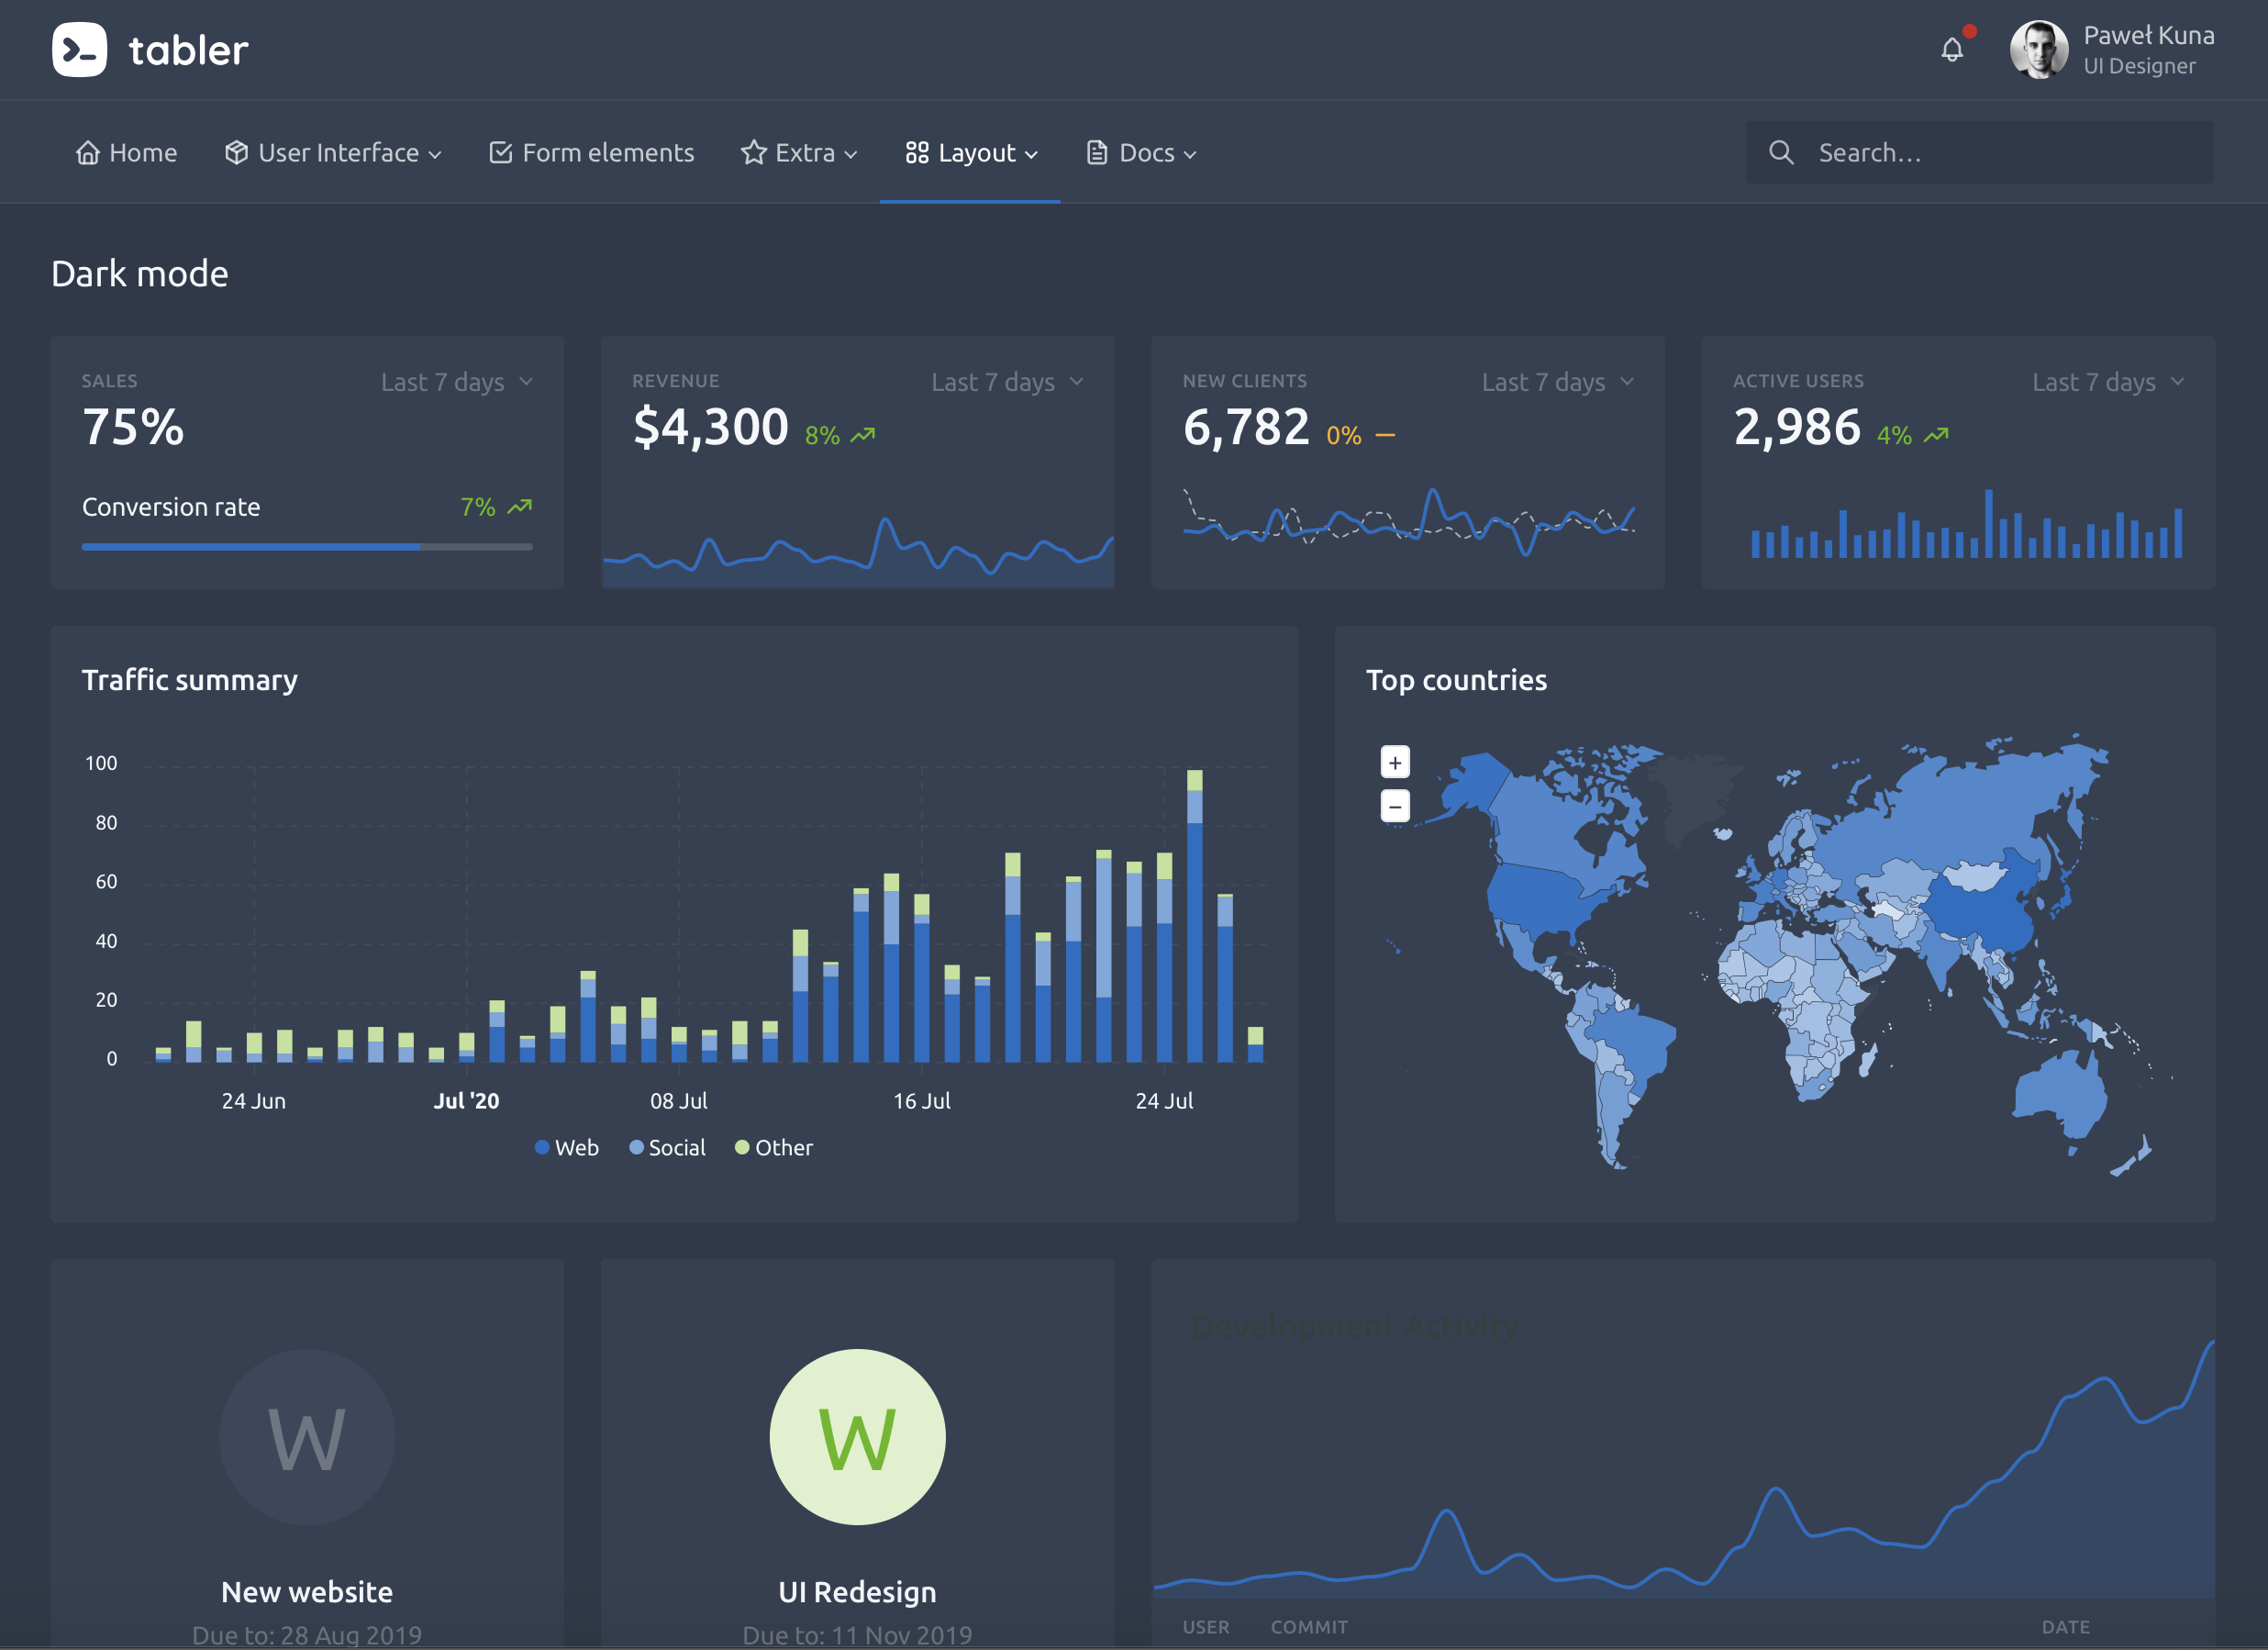
\includegraphics[width=34.33in]{images/practice/tabler-dark} \caption{Tabler dashboard overview}\label{fig:tabler-dark}
\end{figure}

\hypertarget{custom-templates-dependencies}{%
\chapter{Define dependencies}\label{custom-templates-dependencies}}

This is time to start our practical session. As mentionned in the previous chapter, we will focus on the tabler, a tiny Bootstrap 4 dashboard template.
Importantly, what follows is not the description of how to customize tabler but rather provide a R wrapper. Therefore we will not write SASS nore edit the core JavaScript, even though technically possible.

\hypertarget{discover-the-project}{%
\section{Discover the project}\label{discover-the-project}}

The first step of any template adaptation consists in exploring the underlying github repository (if open source) and look for mandatory elements, like CSS/JS dependencies. You would actually proceed similarly for an HTMLWidget.

\begin{figure}
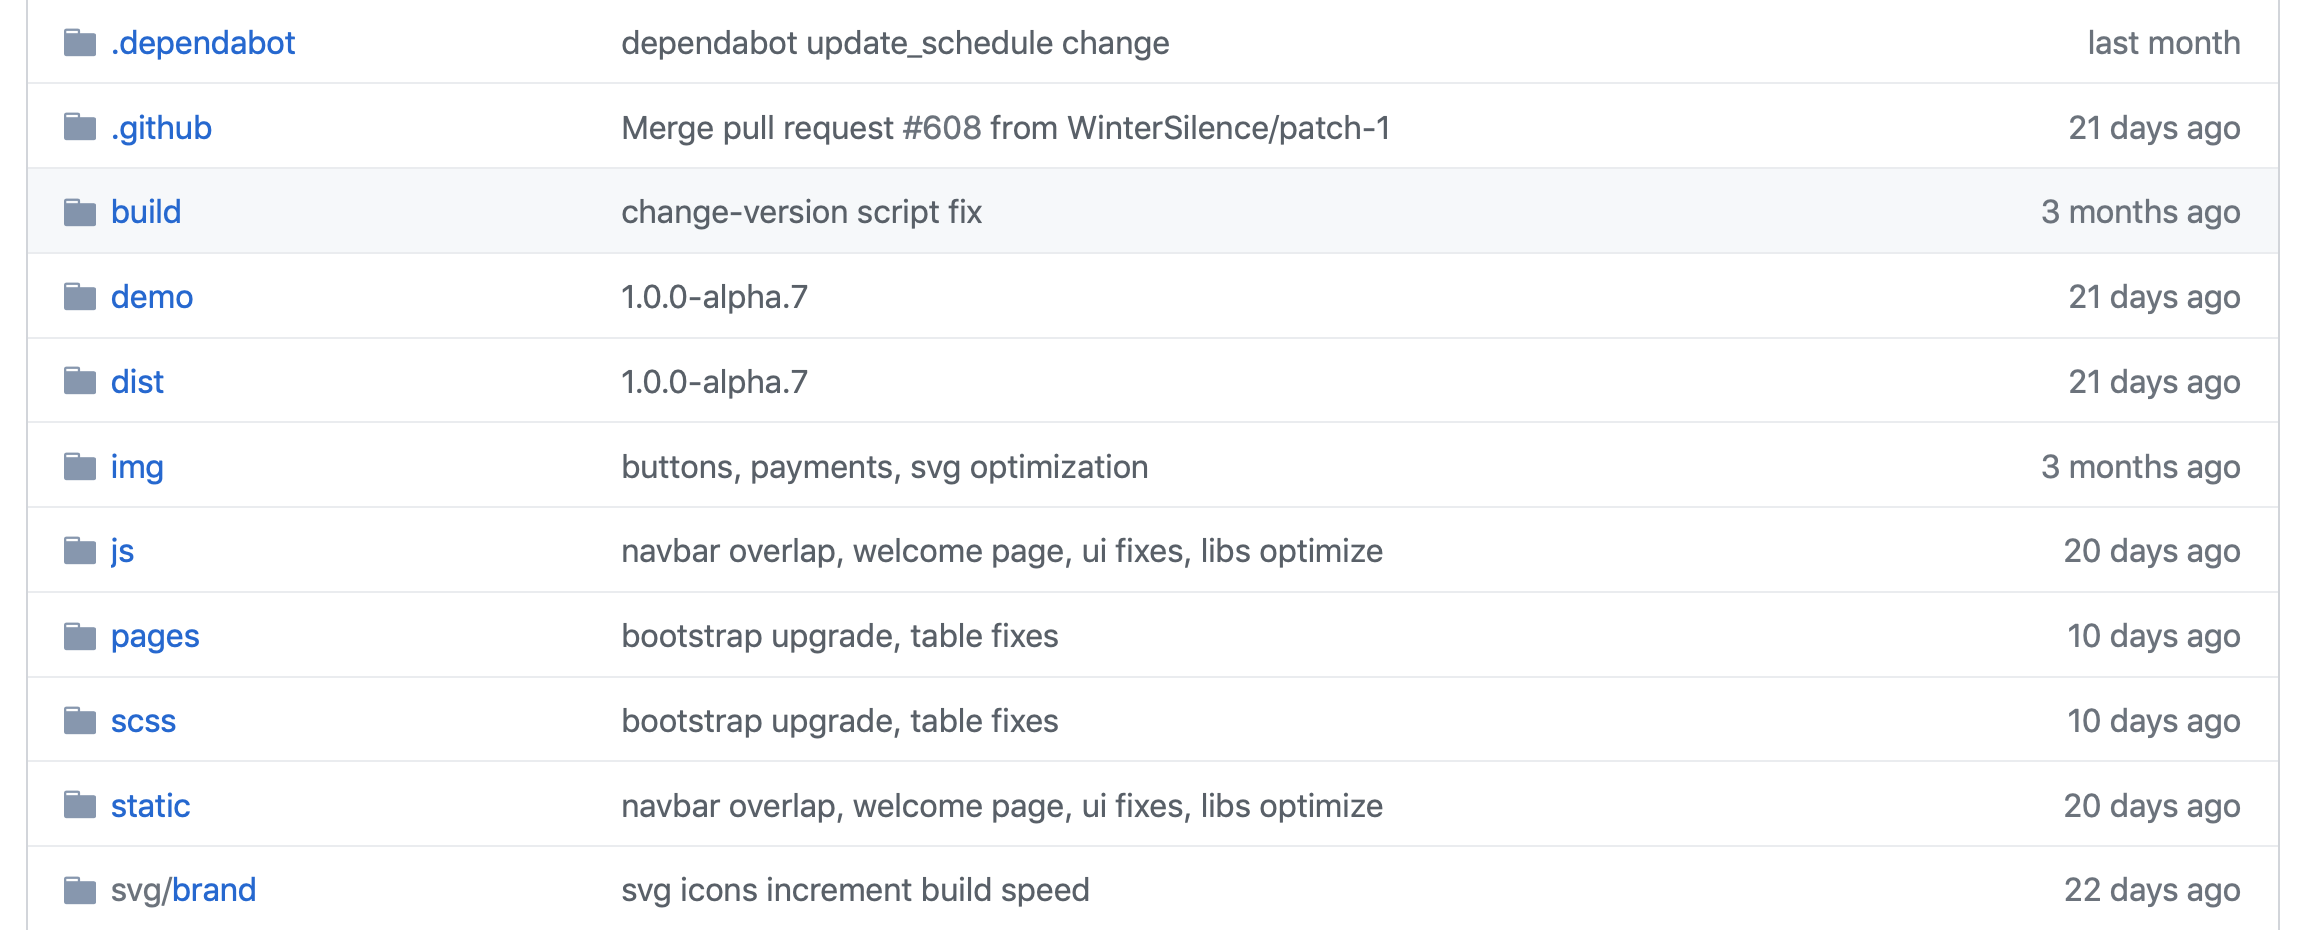
\includegraphics[width=32.03in]{images/practice/tabler-github} \caption{Github project exploration}\label{fig:tabler-github}
\end{figure}

As shown in Figure \ref{fig:tabler-github}, the most important folders are:

\begin{itemize}
\tightlist
\item
  dist: contains CSS and JS files as well as other libraries like Bootstrap and jQuery. In production we seek for minified files since they take less space. It is also a good moment to look at the version of each dependency that might conflict with Shiny
\item
  demo is the website folder used for demonstration purpose. This is our source to explore the template capabilities in depth
\end{itemize}

The scss and build folder are also crucial to the package but as stated previously, customizing tabler is out of the scope of this book. It is already a significant task to adapt a template from a language to another.

\hypertarget{identify-mandatory-dependencies}{%
\section{Identify mandatory dependencies}\label{identify-mandatory-dependencies}}

Now, among all JS/CSS resources, we need to identify the one necessary to the template. Obviously, the Bootstrap 4, jQuery, tabler.min.css and tabler.min.js are key elements, contrary to flag icons which are optional (and take a lot of space). The package size is also to consider if you plan to release the template on CRAN and respect the 5mB maximum limit. By experience, I can tell you this is quite hard to handle.

\hypertarget{custom-templates-skeleton}{%
\chapter{Template skeleton}\label{custom-templates-skeleton}}

\hypertarget{custom-templates-inputs}{%
\chapter{Develop custom input widgets}\label{custom-templates-inputs}}

\hypertarget{how-does-shiny-handle-inputs}{%
\section{How does Shiny handle inputs?}\label{how-does-shiny-handle-inputs}}

\hypertarget{how-to-add-new-input-to-shiny}{%
\section{How to add new input to Shiny?}\label{how-to-add-new-input-to-shiny}}

\hypertarget{custom-templates-testing}{%
\chapter{Testing templates elements}\label{custom-templates-testing}}

\bibliography{book.bib,packages.bib}

\end{document}
